% Options for packages loaded elsewhere
\PassOptionsToPackage{unicode}{hyperref}
\PassOptionsToPackage{hyphens}{url}
%
\documentclass[
  12pt,
]{book}
\usepackage{amsmath,amssymb}
\usepackage{iftex}
\ifPDFTeX
  \usepackage[T1]{fontenc}
  \usepackage[utf8]{inputenc}
  \usepackage{textcomp} % provide euro and other symbols
\else % if luatex or xetex
  \usepackage{unicode-math} % this also loads fontspec
  \defaultfontfeatures{Scale=MatchLowercase}
  \defaultfontfeatures[\rmfamily]{Ligatures=TeX,Scale=1}
\fi
\usepackage{lmodern}
\ifPDFTeX\else
  % xetex/luatex font selection
\fi
% Use upquote if available, for straight quotes in verbatim environments
\IfFileExists{upquote.sty}{\usepackage{upquote}}{}
\IfFileExists{microtype.sty}{% use microtype if available
  \usepackage[]{microtype}
  \UseMicrotypeSet[protrusion]{basicmath} % disable protrusion for tt fonts
}{}
\makeatletter
\@ifundefined{KOMAClassName}{% if non-KOMA class
  \IfFileExists{parskip.sty}{%
    \usepackage{parskip}
  }{% else
    \setlength{\parindent}{0pt}
    \setlength{\parskip}{6pt plus 2pt minus 1pt}}
}{% if KOMA class
  \KOMAoptions{parskip=half}}
\makeatother
\usepackage{xcolor}
\usepackage{color}
\usepackage{fancyvrb}
\newcommand{\VerbBar}{|}
\newcommand{\VERB}{\Verb[commandchars=\\\{\}]}
\DefineVerbatimEnvironment{Highlighting}{Verbatim}{commandchars=\\\{\}}
% Add ',fontsize=\small' for more characters per line
\usepackage{framed}
\definecolor{shadecolor}{RGB}{248,248,248}
\newenvironment{Shaded}{\begin{snugshade}}{\end{snugshade}}
\newcommand{\AlertTok}[1]{\textcolor[rgb]{0.94,0.16,0.16}{#1}}
\newcommand{\AnnotationTok}[1]{\textcolor[rgb]{0.56,0.35,0.01}{\textbf{\textit{#1}}}}
\newcommand{\AttributeTok}[1]{\textcolor[rgb]{0.13,0.29,0.53}{#1}}
\newcommand{\BaseNTok}[1]{\textcolor[rgb]{0.00,0.00,0.81}{#1}}
\newcommand{\BuiltInTok}[1]{#1}
\newcommand{\CharTok}[1]{\textcolor[rgb]{0.31,0.60,0.02}{#1}}
\newcommand{\CommentTok}[1]{\textcolor[rgb]{0.56,0.35,0.01}{\textit{#1}}}
\newcommand{\CommentVarTok}[1]{\textcolor[rgb]{0.56,0.35,0.01}{\textbf{\textit{#1}}}}
\newcommand{\ConstantTok}[1]{\textcolor[rgb]{0.56,0.35,0.01}{#1}}
\newcommand{\ControlFlowTok}[1]{\textcolor[rgb]{0.13,0.29,0.53}{\textbf{#1}}}
\newcommand{\DataTypeTok}[1]{\textcolor[rgb]{0.13,0.29,0.53}{#1}}
\newcommand{\DecValTok}[1]{\textcolor[rgb]{0.00,0.00,0.81}{#1}}
\newcommand{\DocumentationTok}[1]{\textcolor[rgb]{0.56,0.35,0.01}{\textbf{\textit{#1}}}}
\newcommand{\ErrorTok}[1]{\textcolor[rgb]{0.64,0.00,0.00}{\textbf{#1}}}
\newcommand{\ExtensionTok}[1]{#1}
\newcommand{\FloatTok}[1]{\textcolor[rgb]{0.00,0.00,0.81}{#1}}
\newcommand{\FunctionTok}[1]{\textcolor[rgb]{0.13,0.29,0.53}{\textbf{#1}}}
\newcommand{\ImportTok}[1]{#1}
\newcommand{\InformationTok}[1]{\textcolor[rgb]{0.56,0.35,0.01}{\textbf{\textit{#1}}}}
\newcommand{\KeywordTok}[1]{\textcolor[rgb]{0.13,0.29,0.53}{\textbf{#1}}}
\newcommand{\NormalTok}[1]{#1}
\newcommand{\OperatorTok}[1]{\textcolor[rgb]{0.81,0.36,0.00}{\textbf{#1}}}
\newcommand{\OtherTok}[1]{\textcolor[rgb]{0.56,0.35,0.01}{#1}}
\newcommand{\PreprocessorTok}[1]{\textcolor[rgb]{0.56,0.35,0.01}{\textit{#1}}}
\newcommand{\RegionMarkerTok}[1]{#1}
\newcommand{\SpecialCharTok}[1]{\textcolor[rgb]{0.81,0.36,0.00}{\textbf{#1}}}
\newcommand{\SpecialStringTok}[1]{\textcolor[rgb]{0.31,0.60,0.02}{#1}}
\newcommand{\StringTok}[1]{\textcolor[rgb]{0.31,0.60,0.02}{#1}}
\newcommand{\VariableTok}[1]{\textcolor[rgb]{0.00,0.00,0.00}{#1}}
\newcommand{\VerbatimStringTok}[1]{\textcolor[rgb]{0.31,0.60,0.02}{#1}}
\newcommand{\WarningTok}[1]{\textcolor[rgb]{0.56,0.35,0.01}{\textbf{\textit{#1}}}}
\usepackage{longtable,booktabs,array}
\usepackage{calc} % for calculating minipage widths
% Correct order of tables after \paragraph or \subparagraph
\usepackage{etoolbox}
\makeatletter
\patchcmd\longtable{\par}{\if@noskipsec\mbox{}\fi\par}{}{}
\makeatother
% Allow footnotes in longtable head/foot
\IfFileExists{footnotehyper.sty}{\usepackage{footnotehyper}}{\usepackage{footnote}}
\makesavenoteenv{longtable}
\usepackage{graphicx}
\makeatletter
\def\maxwidth{\ifdim\Gin@nat@width>\linewidth\linewidth\else\Gin@nat@width\fi}
\def\maxheight{\ifdim\Gin@nat@height>\textheight\textheight\else\Gin@nat@height\fi}
\makeatother
% Scale images if necessary, so that they will not overflow the page
% margins by default, and it is still possible to overwrite the defaults
% using explicit options in \includegraphics[width, height, ...]{}
\setkeys{Gin}{width=\maxwidth,height=\maxheight,keepaspectratio}
% Set default figure placement to htbp
\makeatletter
\def\fps@figure{htbp}
\makeatother
\setlength{\emergencystretch}{3em} % prevent overfull lines
\providecommand{\tightlist}{%
  \setlength{\itemsep}{0pt}\setlength{\parskip}{0pt}}
\setcounter{secnumdepth}{5}
\usepackage{booktabs}
\ifLuaTeX
  \usepackage{selnolig}  % disable illegal ligatures
\fi
\usepackage[]{natbib}
\bibliographystyle{apalike}
\IfFileExists{bookmark.sty}{\usepackage{bookmark}}{\usepackage{hyperref}}
\IfFileExists{xurl.sty}{\usepackage{xurl}}{} % add URL line breaks if available
\urlstyle{same}
\hypersetup{
  pdftitle={Introduction to Term Structure Models},
  pdfauthor={Jean-Paul Renne},
  hidelinks,
  pdfcreator={LaTeX via pandoc}}

\title{Introduction to Term Structure Models}
\author{Jean-Paul Renne}
\date{2023-12-18}

\usepackage{amsthm}
\newtheorem{theorem}{Theorem}[chapter]
\newtheorem{lemma}{Lemma}[chapter]
\newtheorem{corollary}{Corollary}[chapter]
\newtheorem{proposition}{Proposition}[chapter]
\newtheorem{conjecture}{Conjecture}[chapter]
\theoremstyle{definition}
\newtheorem{definition}{Definition}[chapter]
\theoremstyle{definition}
\newtheorem{example}{Example}[chapter]
\theoremstyle{definition}
\newtheorem{exercise}{Exercise}[chapter]
\theoremstyle{definition}
\newtheorem{hypothesis}{Hypothesis}[chapter]
\theoremstyle{remark}
\newtheorem*{remark}{Remark}
\newtheorem*{solution}{Solution}
\begin{document}
\maketitle

{
\setcounter{tocdepth}{1}
\tableofcontents
}
\newcommand{\bv}[1]{\mathbf{#1}}

\hypertarget{intro}{%
\chapter*{Introduction to Term Structure Models}\label{intro}}

Modeling dynamic term structures serves as a practical and indispensable tool in the realm of finance. It enables investors, institutions, and policymakers to make informed decisions, manage risk effectively, and allocate resources wisely. By understanding how interest rates and yields evolve over time, these models offer a clear lens through which to assess market trends and price financial instruments accurately.

This course has been developed by \href{https://sites.google.com/site/jeanpaulrenne/home}{Jean-Paul Renne}. It is illustrated by R codes using various packages that can be obtained from \href{https://cran.r-project.org}{CRAN}. This \texttt{AEC} package is available on GitHub. To install it, one need to employ the \texttt{devtools} library:

\begin{Shaded}
\begin{Highlighting}[]
\FunctionTok{install.packages}\NormalTok{(}\StringTok{"devtools"}\NormalTok{) }\CommentTok{\# in case this library has not been loaded yet}
\FunctionTok{library}\NormalTok{(devtools)}
\FunctionTok{install\_github}\NormalTok{(}\StringTok{"jrenne/AEC"}\NormalTok{)}
\FunctionTok{library}\NormalTok{(AEC)}
\end{Highlighting}
\end{Shaded}

\textbf{Useful (R) links:}

\begin{itemize}
\item
  Download R:

  \begin{itemize}
  \tightlist
  \item
    R software: \url{https://cran.r-project.org} (the basic R software)
  \item
    RStudio: \url{https://www.rstudio.com} (a convenient R editor)
  \end{itemize}
\item
  Tutorials:

  \begin{itemize}
  \tightlist
  \item
    Rstudio: \url{https://dss.princeton.edu/training/RStudio101.pdf} (by Oscar Torres-Reyna)
  \item
    R: \url{https://cran.r-project.org/doc/contrib/Paradis-rdebuts_en.pdf} (by Emmanuel Paradis)
  \item
    My own tutorial: \url{https://jrenne.shinyapps.io/Rtuto_publiShiny/}
  \end{itemize}
\end{itemize}

\hypertarget{affine-processes}{%
\chapter{Affine processes}\label{affine-processes}}

\hypertarget{Information}{%
\section{Information in the Economy: The ``Factors''}\label{Information}}

\begin{itemize}
\tightlist
\item
  New information at date \(t=1,2,\dots,T\): \(K\)-dimensional \emph{factor} \(w_t\), or \emph{state}.
\item
  Information available at \(t\): \(\underline{w_t} = (w_t,w_{t-1},\dots,w_1)\).
\item
  \(w_t\): random vector, observable, partially observable, or unobservable by the econometrician.
\end{itemize}

\begin{example}[Stock option pricing]
\protect\hypertarget{exm:exStockOption}{}\label{exm:exStockOption}\leavevmode

\begin{itemize}
\tightlist
\item
  Stock option pricing: \(w_t = (y_t, z_t)\) with

  \begin{enumerate}
  \def\labelenumi{\arabic{enumi}.}
  \tightlist
  \item
    \(y_t\): observable vector of (geometric) returns,
  \item
    \(z_t\): regime, unobservable by the econometrician.
  \end{enumerate}
\item
  Term structure of interest rates:
\end{itemize}

\(w_t\): unobservable factor or observable vector of yields or spreads, macroeconomic variables.

\end{example}

\hypertarget{Dynamic}{%
\section{Dynamic Models}\label{Dynamic}}

\begin{itemize}
\tightlist
\item
  Aim: modelling the dynamics of \(w_t\) (historical or risk-neutral, see Chapter @ref(section:PandQ\}).
\item
  Parametric modelling:
  * Choice of a family of conditional probability density functions \(f(w_{t+1}|\underline{w_t},\theta)\), \(\theta\) unknown vector \(\in \Theta\).
  * Equivalently, choice of a conditional \emph{Laplace transforms}:
  \[
  \varphi(u|\underline{w_t},\theta) =
  \mathbb{E}_{\theta}[\exp(u'w_{t+1})|\underline{w_t}], \quad u \in \mathbb{R}^K,
  \]
  or a conditional \emph{log Laplace transforms}:
  \[
  \psi(u|\underline{w_t},\theta) =
  \log\{\mathbb{E}_{\theta}[\exp(u'w_{t+1})|\underline{w_t}]\}, \quad u \in
  \mathbb{R}^K.
  \]
\end{itemize}

\begin{example}[Conditionally Bernoulli process]
\protect\hypertarget{exm:exBenoulli}{}\label{exm:exBenoulli}If \(w_{t+1}|\underline{w_t} \sim {\mathcal{I}} [p(\underline{w_t},\theta)]\), then:
\[
\varphi(u|w_t)=
\mathbb{E}[\exp(u w_{t+1}) \mid \underline{w_t}] = p_t \exp(u) + 1-p_t
\]
with \(p_t = p(w_t, \theta)\).
\end{example}

\begin{example}[Conditionally Bernoulli process]
\protect\hypertarget{exm:exBenoulli2}{}\label{exm:exBenoulli2}If \(w_{t+1}|\underline{w_t} \in {\mathcal{B}}(n, p_t)\), then:
\[
\varphi(u|w_t)=[p_t   \exp(u) + 1-p_t]^n.
\]
\end{example}

\begin{example}[Conditionally Poisson process]
\protect\hypertarget{exm:exPoisson}{}\label{exm:exPoisson}If \(w_{t+1}|\underline{w_t} \sim {\mathcal{P}}(\lambda_t)\), then:
\begin{eqnarray*}
\varphi(u|w_t) & =&   \sum^\infty_{j=0}  \dfrac{1}{j!}  \exp(-\lambda_t) \lambda^j_t   \exp(uj)  = \exp(-\lambda_t) exp[\lambda_t \exp(u)] \\
& =& \exp\{\lambda_t[\exp(u)-1]\}.
\end{eqnarray*}
\end{example}

\begin{example}[Conditionally normal (or Gaussian) process]
\protect\hypertarget{exm:exGaussian}{}\label{exm:exGaussian}If \(w_{t+1}|\underline{w_t} \sim \mathcal{N}\left(m(\underline{w_t},\theta), \Sigma(\underline{w_t},\theta)\right)\), then:

\[
u'w_{t+1}|\underline{w_t} \sim \mathcal{N}\left(u'm(\underline{w_t},\theta), u'\Sigma(\underline{w_t},\theta)u\right).
\]

\[
\Rightarrow
\left\{
\begin{array}{ccc}
\varphi(u|\underline{w_t},\theta) &=& \exp\left[
\begin{array}{l} u'm(\underline{w_t},\theta)+
\frac{1}{2} u'\Sigma(\underline{w_t},\theta)u\end{array}
\right]\\
\psi(u|\underline{w_t},\theta) &=&
u'm(\underline{w_t},\theta) +  \frac{1}{2}
u'\Sigma(\underline{w_t},\theta)u.
\end{array}
\right.
\]
\end{example}

\hypertarget{AffineLaplace}{%
\section{Some Properties of the Laplace Transform}\label{AffineLaplace}}

\begin{itemize}
\item
  \(\varphi(0|\underline{w_t},\theta) = 1\) and \(\psi(0|\underline{w_t},\theta)=0\).
\item
  Defined in a convex set \(E\) (containing \(0\)).
\item
  If the interior of \(E\) is non empty, all the (conditional) moments exist.
\item
  Scalar case:
\item
  Moment of order \(n\):
  \[
  \left[ \begin{array}{l}  \dfrac{\partial^n
  \varphi(u|\underline{w_t},\theta)}{\partial u^n}
  \end{array} \right]_{u=0} = \mathbb{E}_{\theta}[w^n_{t+1}|\underline{w_t}].
  \]
\item
  Cumulant of order \(n\):
  \[
  \left[ \begin{array}{l}  \dfrac{\partial^n
  \psi(u|\underline{w_t},\theta)}{\partial u^n}
  \end{array} \right]_{u=0} = K_n(\underline{w_t},\theta).
  \]
\item
  In particular:
  \[
  \left\{
  \begin{array}{ccc}
  K_1(\underline{w_t},\theta) &=& \mathbb{E}_{\theta}[w_{t+1}|\underline{w_t}]\\
  K_2(\underline{w_t}, \theta) &=& \mathbb{V}ar_{\theta}[w_{t+1}|\underline{w_t}].
  \end{array}
  \right.
  \]
\end{itemize}

\varphi\$ and \(\psi\) are respectively called conditional \textbf{moment} and \textbf{cumulant} generating function.

\begin{itemize}
\tightlist
\item
  Multivariate case:
  \begin{eqnarray*}
  \left[\begin{array}{l}  \dfrac{\partial \psi}{\partial
  u} (u|\underline{w_t},\theta)  \end{array} \right]_{u=0} &=& \mathbb{E}_{\theta}[w_{t+1}|\underline{w_t}] \\
  \left[\begin{array}{l}  \dfrac{\partial^2
  \psi}{\partial u\partial u'} (u|\underline{w_t},\theta)  \end{array}
  \right]_{u=0} &=& \mathbb{V}ar_{\theta}[w_{t+1}|\underline{w_t}].
  \end{eqnarray*}
\end{itemize}

\begin{example}[Conditionally normal (or Gaussian) process]
\protect\hypertarget{exm:exGaussian}{}\label{exm:exGaussian}

See Example \ref{exm:exGaussian}

\begin{itemize}
\item
  Scalar case
\item
  \(\psi(u|\underline{w_t},\theta)=u m(\underline{w_t},\theta) +  \frac{1}{2}u^2\sigma^2(\underline{w_t},\theta)\).
\item
  \(\left[\begin{array}{l} \dfrac{\partial \psi}{\partial u} (u|\underline{w_t},\theta) \end{array} \right]_{u=0} = m(\underline{w_t},\theta)\).
\item
  \(\left[\begin{array}{l} \dfrac{\partial^2 \psi}{\partial u^2} (u|\underline{w_t},\theta) \end{array} \right]_{u=0} = \sigma^2(\underline{w_t},\theta)\).
\item
  Multidimensional case
\item
  \(\psi(u|\underline{w_t},\theta)=u' m(\underline{w_t},\theta) +  \frac{1}{2}u'\Sigma(\underline{w_t},\theta)u\).
\item
  \(\left[\begin{array}{l} \dfrac{\partial \psi}{\partial u} (u|\underline{w_t},\theta) \end{array} \right]_{u=0} = m(\underline{w_t},\theta)\).
\item
  \(\left[\begin{array}{l} \dfrac{\partial^2 \psi}{\partial u\partial u'} (u|\underline{w_t},\theta) \end{array} \right]_{u=0} = \Sigma(\underline{w_t},\theta)\).
\item
  In both cases, cumulants of order \(>2\) equal to \(0\).
\end{itemize}

\end{example}

\begin{itemize}
\item
  If \(w_t=(w'_{1t},w'_{2t})'\) \(, u=(u'_1, u'_2)'\):
  \begin{eqnarray*}
  \mathbb{E}_{\theta}[\exp(u'_1 w_{1,t+1}|\underline{w_t})&=&\varphi(u_1,0|\underline{w_t},\theta)] \\
  \mathbb{E}_{\theta}[\exp(u'_2 w
  _{2,t+1}|\underline{w_t})&=&\varphi(0,u_2|\underline{w_t},\theta)].
  \end{eqnarray*}
\item
  If \(w_t=(w'_{1t},w'_{2t})'\), and if \(w_{1t}\) and \(w_{2t}\) are conditionally independent:
  \begin{eqnarray*}
  \varphi(u|\underline{w_t},\theta) &=&
  \varphi(u_1,0|\underline{w_t},\theta)\times\varphi(0,u_2|\underline{w_t},\theta) \\
  \psi(u|\underline{w_t},\theta) &=&
  \psi(u_1,0|\underline{w_t},\theta)+\psi(0,u_2|\underline{w_t},\theta).
  \end{eqnarray*}
\item
  if \(w_{1t}\) and \(w_{2t}\) have the same size and if
  \[
  \varphi(u_1, u_2|\underline{w_t},\theta) = \mathbb{E}_\theta[\exp(u'_1 w_{1, t+1} + u'_2 w_{2,t+1}|\underline{w_t}],
  \]
  then the conditional Laplace transform of \(w_{1, t+1} + w_{2, t+1}\) given
  \(\underline{w_t}\) is \(\varphi(u, u|\underline{w_t},\theta)\).

  \begin{itemize}
  \tightlist
  \item
    If \(w_{1t}\) and \(w_{2t}\) are conditionally independent,
    same size, the conditional Laplace transform and Log-Laplace
    transform of \(w_{1,t+1}+w_{2,t+1}\) are respectively:
    \[
    \varphi(u,0|\underline{w_t},\theta)\times \varphi(0,
    u|\underline{w_t},\theta)
    \]
    and
    \[
    \psi(u,0|\underline{w_t},\theta)+ \psi(0,
    u|\underline{w_t},\theta).
    \]
  \end{itemize}
\end{itemize}

\begin{lemma}[Conditional zero probability for non-negative processes]
\protect\hypertarget{lem:lemMass}{}\label{lem:lemMass}If \(w_t\) is univariate and nonnegative its (conditional)
Laplace transform \(\varphi_t(u) = \mathbb{E}_t[\exp(u w_{t+1})]\) is defined
for \(u \leq 0\) and
\[
\mathbb{P}_t(w_{t+1} = 0) = \lim_{u\rightarrow - \infty} \varphi_t(u).
\]
\end{lemma}

\begin{proof}
We have \(\varphi_t(u) = \mathbb{P}_t(w_{t+1} = 0) + \int_{w_{t+1}> 0} \exp(u w_{t+1}) d\mathbb{P}_t(w_{t+1})\). The Lebesgue theorem ensures that the last integral converges to zero when \(u\) goes to \(-\infty\).
\end{proof}

\begin{lemma}[Conditional zero probability for non-negative multivariate processes]
\protect\hypertarget{lem:lemPetitLemme}{}\label{lem:lemPetitLemme}Assume that:
* \(w_{1,t}\) is valued in \(\mathbb{R}^{d}\) (\(d \geq 1\)),
* \(w_{2,t}\) is valued in \(\mathbb{R}^+ = [0, + \infty )\),
* \(\mathbb{E}_t \left[ \exp \left( u_1 ' w_{1,t+1} + u_2 w_{2,t+1} \right) \right]\) exists for a given \(u_1\) and \(u_2 \leq 0\).

Then, we have:
\begin{equation}
\mathbb{E}_t \left[ \exp( u_1 ' w_{1,t+1})  \textbf{1}_{\{w_{2,t+1} = 0 \}} \right] =  \underset{u_2 \rightarrow -\infty}{\lim} \mathbb{E}_t \left[ \exp( u_1 ' w_{1,t+1} + u_2   w_{2,t+1} )  \right].\label{eq:petitlemme}
\end{equation}
\end{lemma}

\begin{proof}
We have that
\begin{eqnarray*}
&&\underset{u_2 \rightarrow -\infty}{\lim} \mathbb{E}_t \left[ \exp( u_1 ' w_{1,t+1} + u_2   w_{2,t+1} )  \right] \\
&=& \mathbb{E}_t \left[ \exp( u_1 ' w_{1,t+1})   \textbf{1}_{\{w_{2,t+1} = 0 \}} \right] +\\
&& \underset{u_2 \rightarrow -\infty}{\lim}   \mathbb{E}_t \left[ \exp( u_1 ' w_{1,t+1} + u_2   w_{2,t+1} )  \textbf{1}_{\{w_{2,t+1} > 0 \}}  \right] ,
\end{eqnarray*}
and since in the second term on the right-hand side \(\exp(u_2 w_{2,t+1}) \textbf{1}_{\{w_{2,t+1} > 0 \}} \rightarrow 0\) when \(u_2 \rightarrow -\infty\), relation \eqref{eq:petitlemme} is a consequence of the Lebesgue theorem.
\end{proof}

\hypertarget{AffineCar}{%
\section{Affine (or Car) Processes}\label{AffineCar}}

\begin{definition}[Affine process of order 1]
\protect\hypertarget{def:Car1}{}\label{def:Car1}A multivariate process \(w_{t+1}\) is Affine of order 1 {[}or \(Car(1)\){]} if
\[
\varphi_t(u)=\mathbb{E}_t[\exp(u'w_{t+1})]=\exp[a(u)'w_t+b(u)]
\]
for some functions \(a(.)\) and \(b(.)\). These functions are univariate if \(w_{t+1}\) (and therefore \(u\)) is scalar.
\end{definition}

\begin{itemize}
\tightlist
\item
  \emph{Car} stands for \emph{Compound auto-regressive}.
\item
  \(a(.)\) and b(.) may be deterministic functions of time.
\end{itemize}

\begin{example}[Univariate AR(1) Gaussian process]
\protect\hypertarget{exm:GAR1}{}\label{exm:GAR1}If \(w_{t+1}|\underline{w_t} \sim \mathcal{N}(\nu+\rho w_t, \sigma^2)\), then:
\[
\varphi_t(u) = \exp\left(
\begin{array}{l}
u \rho w_t + u \nu + u^2  \frac{\sigma^2}{2}
\end{array}
\right) = \exp[a(u)'w_t+b(u)],
\]
\[
\mbox{with }\left\{
\begin{array}{ccc}
a(u) &=& u \rho\\
b(u) &=& u \nu + u^2  \dfrac{\sigma^2}{2}.
\end{array}
\right.
\]
\end{example}

\begin{example}[Gaussian VAR]
\protect\hypertarget{exm:GVAR1}{}\label{exm:GVAR1}If \(w_{t+1}|\underline{w_t} \sim \mathcal{N}(\mu+\Phi w_t, \Sigma)\), then:
\[
\varphi_t(u) = \exp\left(
\begin{array}{l}
u' (\mu + \Phi  w_t)  +  \frac{1}{2} u' \Sigma u
\end{array}
\right) = \exp[a(u)'w_t+b(u)],
\]
\[
\mbox{with }\left\{
\begin{array}{ccl}
a(u) &=& \Phi'u\\
b(u) &=& u' \mu +  \frac{1}{2} u' \Sigma u = u' \mu + \frac{1}{2}(u \otimes u)' vec(\Sigma).
\end{array}
\right.
\]
\end{example}

\begin{example}[Quadratic Gaussian process]
\protect\hypertarget{exm:QGVAR1}{}\label{exm:QGVAR1}\leavevmode

\begin{itemize}
\tightlist
\item
  Consider \(w_t = (x'_t,vec(x_t x_t')')'\), where \(x_t\) is a \(n\)-dimensional vector following a Gaussian VAR(1), i.e.
  \[
  x_{t+1}|\underline{w_t} \sim \mathcal{N}(\mu+\Phi x_t, \Sigma).
  \]

  \begin{itemize}
  \tightlist
  \item
    If \(u = (v,V)\) where \(v \in \mathbb{R}^n\) and \(V\) a square symmetric matrix of size \(n\), we have:
    \begin{eqnarray*}
      \varphi_t(u) &=& \mathbb{E}_t\big\{\exp\big[(v',vec(V)')\times w_{t+1}\big]\big\} \\
      & =& \exp \left\{a_1(v,V)'x_t +vec(a_2(v,V))' vec(x_t'x_t) + b(v,V) \right\},
      \end{eqnarray*}
    where:
    \begin{eqnarray*}\label{eq:laplaceZ}
          a_2(u) & = & \Phi'V (I_n - 2\Sigma V)^{-1} \Phi \nonumber \\
          a_1(u) & = & \Phi'\left[(I_n-2V\Sigma)^{-1}(v+2V\mu)\right] \nonumber \\
          b(u) & = & u'(I_n - 2 \Sigma V)^{-1}\left(\mu + \frac{1}{2} \Sigma v\right) +\\
          && \mu'V(I_n - 2 \Sigma V)^{-1}\mu - \frac{1}{2}\log\big|I_n - 2\Sigma V\big|.
      \end{eqnarray*}
  \end{itemize}
\end{itemize}

\end{example}

\begin{proof}
We have:
\begin{eqnarray*}
&&\mathbb{E}_t(\exp(v' x_{t+1} + vec(V)'vec(x_{t+1} x_{t+1}'))) \\
&=& \mathbb{E}_t[\exp(v' (\mu + \Phi x_t + \Sigma^{1/2}\varepsilon_{t+1}) + \\
&& vec(V)'vec((\mu + \Phi x_t + \Sigma^{1/2}\varepsilon_{t+1}) (\mu + \Phi x_t + \Sigma^{1/2}\varepsilon_{t+1})'))] \\
&=& \exp[v' (\mu + \Phi x_t) + vec(V)'vec\{(\mu + \Phi x_t)(\mu + \Phi x_t)'\}] \times \\
&& \mathbb{E}_t[\exp(v'\Sigma^{1/2}\varepsilon_{t+1} +2\underbrace{ vec(V)' vec\{(\mu + \Phi x_t)(\varepsilon_{t+1}'{\Sigma^{1/2}}')\}}_{=(\mu + \Phi x_t)'V\Sigma^{1/2}\varepsilon_{t+1}} +\\
&& \underbrace{vec(V)'vec\{(\Sigma^{1/2}\varepsilon_{t+1})(\Sigma^{1/2}\varepsilon_{t+1})'}_{=\varepsilon_{t+1}'{\Sigma^{1/2}}'V\Sigma^{1/2}\varepsilon_{t+1}}\}]
\end{eqnarray*}
Lemma @ref(lemma:Quadr\} can be used to compute the previous conditional expectation, with \(\lambda = {\Sigma^{1/2}}'(v + 2 V'(\mu + \Phi x_t))\). Some algebra then leads to the result.
\end{proof}

\begin{example}[Autoregressive gamma process, ARG(1)]
\protect\hypertarget{exm:ARG1}{}\label{exm:ARG1}

An ARG process is defined as follows:
\[
\frac{w_{t+1}}{\mu} \sim \gamma(\nu+z_t) \quad \mbox{where} \quad z_t \sim \mathcal{P} \left( \frac{\rho w_t}{\mu} \right),
\]
with \(\nu\), \(\mu\), \(\rho > 0\). (Alternatively \(z_t \sim {\mathcal{P}}(\beta w_t)\), with \(\rho = \beta \mu\).)

We have:
\(\varphi_t(u) = exp \left[ \begin{array}{l}  \dfrac{\rho u}{1-u \mu} w_t - \nu \log(1-u \mu)\end{array} \right], u < \dfrac{1}{\mu}\).

That is: \(\varphi_t(u) = \exp[a(u)'w_t+b(u)]\) with
\[
\left\{
\begin{array}{ccc}
a(u) &=&  \dfrac{\rho u}{1-u \mu}\\
b(u) &=& -\nu  
\log(1-u \mu).
\end{array}
\right.
\]

\begin{proof}
Given \(\underline{w_t}\), we have \(z_t \sim {\mathcal P}\left( \begin{array}{l} \frac{\rho w_t} {\mu} \end{array}\right)\). We have:
\begin{eqnarray*}
\mathbb{E}[\exp(u w_{t+1})|\underline{w_t}] &=& \mathbb{E}\left\{\mathbb{E}\left[\exp \left(u \mu  \frac{w_{t+1}}{\mu}\right)|\underline{w_t}, \underline{z}_t\right]\underline{w_t}\right\}\\
&=& \mathbb{E}[(1-u\mu)^{-(\nu+z_t)}|\underline{w_t}] \\
&=& (1-u\mu)^{-\nu}\mathbb{E}\{\exp[-z_t   \log(1-u\mu)]|\underline{w_t}\} \\
&=& (1-u\mu)^{-\nu} \exp \left\{\frac{\rho w_t}{\mu}[\exp(-\log(1-u\mu)] -  \frac{\rho w_t}{\mu}\right\}\\
&=& exp\left[ \begin{array}{l}  \frac{\rho u w_t}{1-u\mu} - \nu   \log(1-u\mu)  \end{array}\right],
\end{eqnarray*}
using the fact that the L.T. of \(\gamma(\nu)\) is \((1-u)^{-\nu}\)
and that the L.T. of \({\mathcal P}(\lambda)\) is \(\exp[\lambda(exp(u)-1)]\).
\end{proof}

\href{https://jrenne.shinyapps.io/Affine/}{Web-interface illustration (``ARG'' panel)}

\begin{itemize}
\tightlist
\item
  This is a positive process.
\item
  We have:
  \[
    \left\{
    \begin{array}{ccc}
    \mathbb{E}(w_{t+1}|\underline{w_t}) &=& \nu \mu + \rho w_t \\
    \mathbb{V}ar(w_{t+1}|\underline{w_t}) &=& \nu \mu^2 + 2 \mu \rho w_t.
    \end{array}
    \right.
    \]
\item
  We have:
  \[
    w_{t+1}=\nu\mu+\rho w_t+\varepsilon_{t+1},
    \]
  where \(\varepsilon_{t+1}\) is a martingale difference \(\Rightarrow\) \(w_{t+1}\) is a weak \(AR(1)\).

  \begin{itemize}
  \tightlist
  \item
    \(ARG_0(1)\) process \citep{zarg_2017}: \(\nu = 0\) and \(\beta w_t\) replaced by \(\alpha + \beta w_t\), i.e.:
    \begin{equation}
      \frac{w_{t+1}}{\mu} \sim \gamma(z_t),\quad z_t \sim {\mathcal{P}}(\alpha + \beta w_t)\label{eq:ARG0}
      \end{equation}
    \[
      \Rightarrow \varphi_t(u) = exp \left[\frac{\beta \mu u}{1-u \mu} w_t + \frac{\alpha \mu u}{1-u \mu}
    \right].
    \]
    Point mass at zero with conditional probability \(exp(-\alpha - \beta w_t)\), 0 is absorbing if \(\alpha = 0\).
  \end{itemize}
\end{itemize}

\begin{Shaded}
\begin{Highlighting}[]
\FunctionTok{library}\NormalTok{(TSModels)}
\NormalTok{W }\OtherTok{\textless{}{-}} \FunctionTok{simul.ARG}\NormalTok{(}\DecValTok{300}\NormalTok{,}\AttributeTok{mu=}\NormalTok{.}\DecValTok{5}\NormalTok{,}\AttributeTok{nu=}\DecValTok{0}\NormalTok{,}\AttributeTok{rho=}\NormalTok{.}\DecValTok{9}\NormalTok{,}\AttributeTok{alpha=}\NormalTok{.}\DecValTok{1}\NormalTok{)}
\FunctionTok{plot}\NormalTok{(W,}\AttributeTok{type=}\StringTok{"l"}\NormalTok{)}
\end{Highlighting}
\end{Shaded}

\begin{figure}
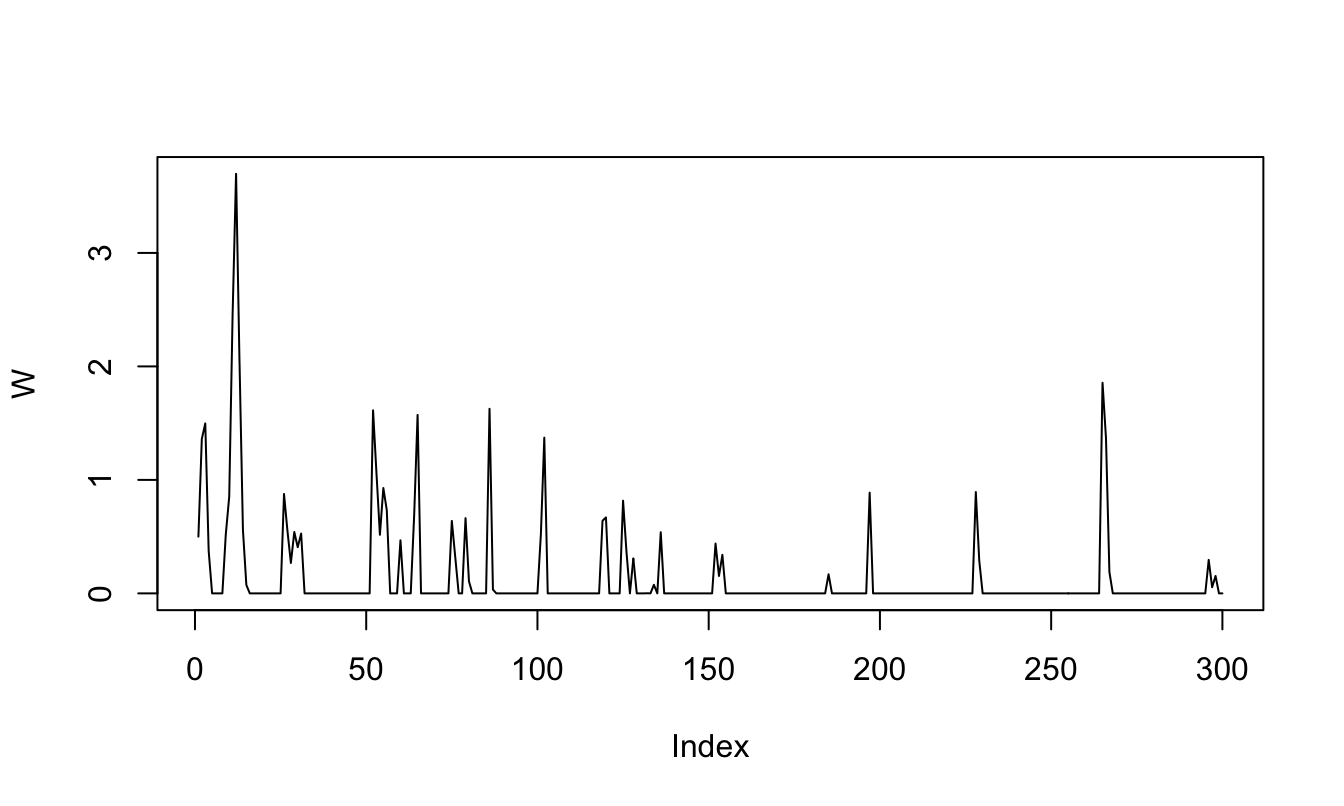
\includegraphics[width=0.95\linewidth]{TSM_files/figure-latex/simARG0-1} \caption{Simulation of an ARG0 processes.}\label{fig:simARG0}
\end{figure}

\end{example}

\begin{example}[Compound Poisson process]
\protect\hypertarget{exm:CompoundPoisson}{}\label{exm:CompoundPoisson}

Consider the following process:
\[\frac{w_{t+1}}{\gamma} = z_{t+1} + \varepsilon_{t+1},
\]
where:
* \(z_{t+1}\) and \(\varepsilon_{t+1}\) conditionally independent,
* \(z_{t+1} \sim {\mathcal B} \left( \begin{array}{l}  \frac{w_t}{\gamma}, \pi \end{array} \right)\),
* \(\varepsilon_{t+1} \sim {\mathcal P}(\lambda)\),
* \(\gamma > 0\), \(0 < \pi< 1\), \(\lambda > 0\).

This process is valued in \(\{j \gamma, j \in \mathbb{N}, \gamma \in \mathbb{R}^+\}\) and we have:
\[
\varphi_t(u) = exp\left\{
\begin{array}{l}
 \dfrac{w_t}{\gamma}   \log[\pi  
exp(u\gamma)+1-\pi]-\lambda[1-exp(u \gamma)]
\end{array}
\right\},
\]
with
\[
\left\{
\begin{array}{ccl}
a(u)&=& \frac{1}{\gamma}   \log[\pi   \exp(u
\gamma)+1-\pi],\\
b(u) &=& -\lambda[1-exp(u \gamma)].
\end{array}
\right.
\]

\begin{itemize}
\tightlist
\item
  We have: \(w_{t+1} = \pi w_t + \lambda \gamma + \eta_{t+1}\), where \(\eta_{t+1}\) is a
  martingale difference.
\end{itemize}

\href{https://jrenne.shinyapps.io/Affine/}{Web-interface illustration (``Compound Poisson'' panel)}

\begin{Shaded}
\begin{Highlighting}[]
\FunctionTok{library}\NormalTok{(TSModels)}
\NormalTok{W }\OtherTok{\textless{}{-}} \FunctionTok{simul.compound.poisson}\NormalTok{(}\DecValTok{100}\NormalTok{,}\AttributeTok{Gamma=}\NormalTok{.}\DecValTok{5}\NormalTok{,}\AttributeTok{Pi=}\FloatTok{0.5}\NormalTok{,}\AttributeTok{lambda=}\NormalTok{.}\DecValTok{9}\NormalTok{)}
\FunctionTok{plot}\NormalTok{(W,}\AttributeTok{type=}\StringTok{"l"}\NormalTok{)}
\end{Highlighting}
\end{Shaded}

\begin{figure}
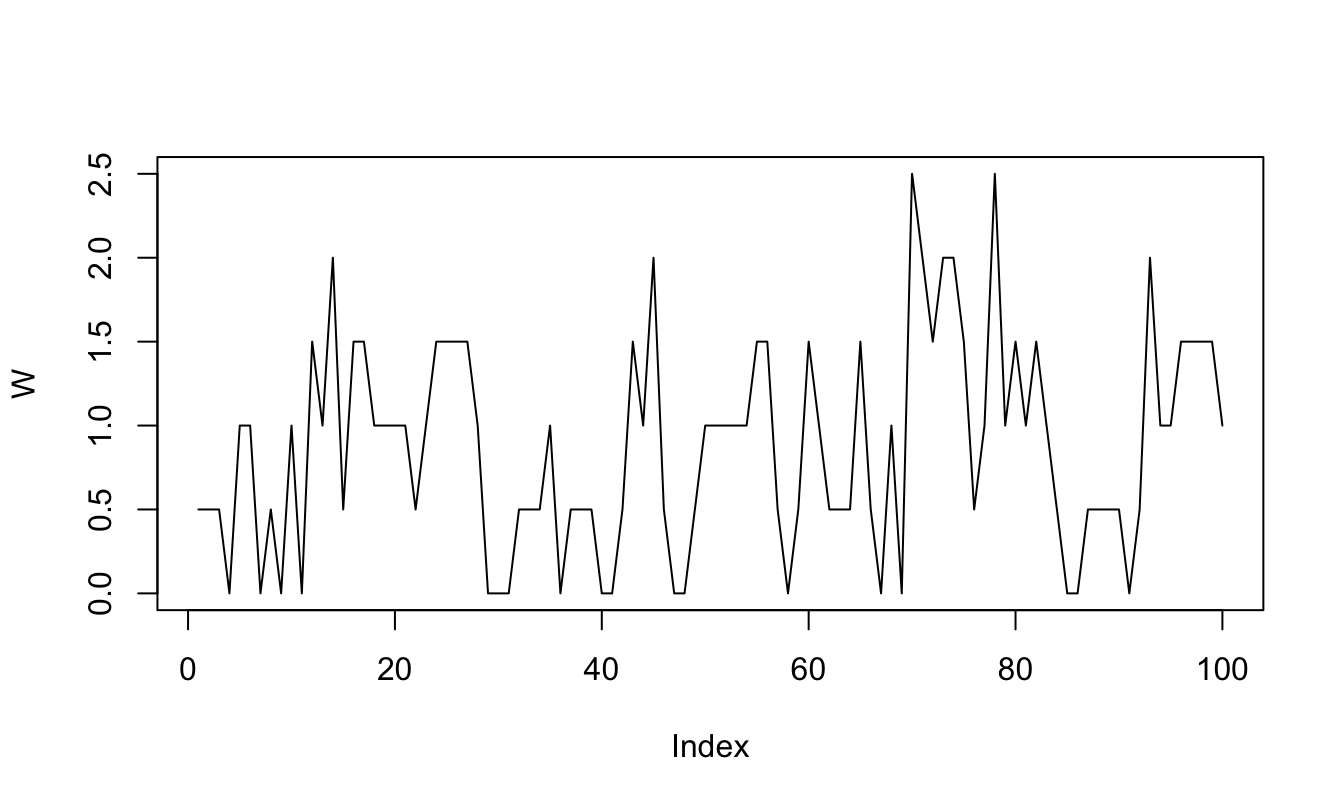
\includegraphics[width=0.95\linewidth]{TSM_files/figure-latex/simCPoisson-1} \caption{Simulation of a Compound Poisson  process.}\label{fig:simCPoisson}
\end{figure}

\end{example}

\hypertarget{CarProcesses}{%
\section{Affine (or Car) processes}\label{CarProcesses}}

\begin{definition}[Affine process of order p]
\protect\hypertarget{def:Carp}{}\label{def:Carp}A multivariate process \(w_{t+1}\) is affine of order \(p\) {[}or \(Car(p)\){]} if
\[
\varphi_t(u)=\mathbb{E}_t[\exp(u' w_{t+1})]=\exp[a_1(u)'w_t+\dots+a_p(u)'w_{t+1-p}+b(u)].
\]
\end{definition}

\textbf{Remarks:}

\begin{itemize}
\item
  If \(w_t\) is \(Car(p)\), then \(W_t = [w_t', w_{t-1}',\dots,w_{t-p+1}']'\) is \(Car(1)\).
\item
  Without loss of generality we can assume \(p = 1\).
\end{itemize}

\begin{proof}
We have:
\begin{eqnarray*}
\mathbb{E}_t[\exp(u'W_{t+1})] &=& \mathbb{E}_t[\exp(u'_1 w_{t+1}+u'_2 w_t+\dots+u'_p w_{t-p+2})] \\
&=& \exp(u'_2 w_t+\dots+u'_p w_{t-p+2})\mathbb{E}_t[\exp(u'_1 w_{t+1})] \\
&=& \exp(u'_2 w_t+\dots+u'_p w_{t-p+2}+a'_1(u_1)
w_t  +\dots+a'_p(u_1)w_{t+1-p}+b(u_1)) \\
&=& \exp[A(u)'W_t+B(u)],
\end{eqnarray*}

with \(A(u)' = [u'_2+a'_1(u_1),\dots,u'_p+a'_{p-1}(u_1), a'_p(u_1)]\) and \(B(u) = b(u_1)\).
\end{proof}

\hypertarget{an-important-particular-case}{%
\subsection{An important particular case}\label{an-important-particular-case}}

\begin{definition}[Univariate Index Affine of order p]
Let \(exp[a(u)w+b(u)]\) be the L.T. of a univariate Affine process of order 1, the process \(w_{t+1}\) is an \{\it Index-Affine\} process of order \(p\) if:
\[
\varphi_t(u)=\mathbb{E}_t[\exp(u w_{t+1})]=\exp[a(u)(\beta_1 w_t+\dots+\beta_p
w_{t+1-p})+b(u)].
\]
\end{definition}

\begin{example}[Gaussian AR(p) process]
\protect\hypertarget{exm:ARp}{}\label{exm:ARp}Extends Example \ref{exm:GAR1}
\begin{eqnarray*}
\varphi_t(u) &=& \exp \left[ u \rho (\beta_1 w_t+\dots+\beta_p w_{t+1-p})+u\nu + u^2  \frac{\sigma^2}{2}\right]\\
w_{t+1} &=& \nu + \varphi_1 w_t +\dots+ \varphi_p w_{t+1-p}+\sigma \varepsilon_{t+1},\quad \varepsilon_{t+1} \sim i.i.d. \mathcal{N}(0,1),
\end{eqnarray*}
with \(\varphi_i = \rho \beta_i\).
\end{example}

\begin{example}[ARG(p) process (positive)]
\protect\hypertarget{exm:ARGp}{}\label{exm:ARGp}Extends Example \ref{exm:ARG1}

\begin{eqnarray*}
\varphi_t(u) &=& \exp\left[\frac{\rho u}{1-u \mu} (\beta_1 w_t+\dots+\beta_p w_{t+1-p})-\nu  \log(1-u\mu)\right],\\
w_{t+1} &=& \nu\mu + \varphi_1 w_t +\dots+ \varphi_p w_{t+1-p}+\varepsilon_{t+1},
\end{eqnarray*}
with \(\varphi_i = \rho \beta_i\) and where \(\varepsilon_{t+1}\) is a martingale difference.
\end{example}

\hypertarget{Markov}{%
\section{Affine (or Car) processes, Markov Chains}\label{Markov}}

\begin{itemize}
\item
  Notations
\item
  \(e_j\) denotes the \(j^{th}\) column of \(Id_J\), \(j=1,\dots,J\).
\item
  \(\pi(e_i, e_j) = \mathbb{P}(z_{t+1}=e_j | z_t=e_i)\).
\item
  With these notations:
  \[
  \mathbb{E}[\exp(v'z_{t+1})|z_t=e_i,\underline{z_{t-1}}] = \sum^J_{j=1} \exp(v'e_j)\pi (e_i, e_j),
  \]
\item
  That is:
  \[
  \varphi_t(v) = exp[a_z(v)'z_t],
  \]
  with
  \[
  a_z(v)= \left[ \begin{array}{l} \log \left(
  \begin{array}{l}  \sum^J_{j=1} \exp(v'e_j)  \pi(e_1,
  e_j) \end{array} \right)\\
  \vdots\\
  \log \left(
  \begin{array}{l}  \sum^J_{j=1} \exp(v'e_j)  \pi(e_J,
  e_j) \end{array} \right)
  \end{array}\right].
  \]
\end{itemize}

\href{https://jrenne.shinyapps.io/Affine/}{Web-interface illustration (``Markov-Switching'' panel)}

\hypertarget{stoch}{%
\section{AFFINE (OR Car) PROCESSES, Stochastic parameters univariate affine processes}\label{stoch}}

\begin{itemize}
\item
  A univariate affine dynamics based on:
  \[
  \mathbb{E}_t   \exp(u y_{t+1}) = \exp[a_0(u)y_t+b_0(u)\delta],
  \]
  where \(\delta = (\delta_1,\dots,\delta_m)' \in \mathcal{D}\), can be generalized to the case of a stochastic \(\delta\).
\item
  More precisely assuming:
  \[
  \mathbb{E}[\exp(u y_{t+1})|\underline{y_t}, \underline{z_{t+1}}] = \exp[a_0(u)y_t+b_0(u)'\Lambda z_{t+1}],
  \]
  where \(\Lambda\) is a \((m\times k)\) matrix, with \(\Lambda z_{t+1} \in \mathcal{D}\), then:
  \[
  \mathbb{E}[\exp(v' z_{t+1})|\underline{y_t}, \underline{z_{t}}] = \exp[a_1(v)'z_t+b_1(v)],
  \]
  \(\Rightarrow\) \(w_{t+1} = (y_{t+1}, z'_{t+1})'\) is affine.
\end{itemize}

\begin{proof}
We have:
\begin{eqnarray*}
&&\mathbb{E}[\exp(u y_{t+1}+v'z_{t+1})|\underline{y_t}, \underline{z_{t}}] \\
&=& \mathbb{E}\{\exp(v' z_{t+1})\mathbb{E}[\exp(u y_{t+1})|\underline{y_t},
\underline{z_{t+1}}]|\underline{y_t}, \underline{z_{t}} \} \\
&=& \mathbb{E}\{\exp[a_0(u) y_{t}+b_0(u)'\Lambda z_{t+1}+v'z_{t+1}]|\underline{y_t},
\underline{z_{t}} \} \\
&=& \exp\{ a_0(u) y_{t}+a_1[\Lambda' b_0(u)+v]'z_t+b_1 [\Lambda' b_0(u)+v]\}.
\end{eqnarray*}
\end{proof}

\begin{example}[Gaussian AR(p)]
\protect\hypertarget{exm:extendedARp}{}\label{exm:extendedARp}

Extends Example \ref{exm:ARp}

\begin{itemize}
\item
  Notations: \(b_0(u) = \left(u, \; \frac{u^2}{2}\right)'\) and \(\delta = (\nu,\sigma^2)' \in \mathcal{D}=\mathbb{R} \times \mathbb{R}^+\).
\item
  \(\delta\) (vector of conditional mean and variance) can be replaced by \ldots{}
\item
  \(\left( \begin{array}{l} z_{1,t+1} \\ z_{2,t+1} \end{array} \right)\), where \(z_{1,t+1}\) and \(z_{2,t+1}\) are independent AR(1) --see Example \ref{exm:GAR1}-- and
  ARG(1) --see Example \ref{exm:ARG1}-- processes respectively.
\item
  \(\left( \begin{array}{ll} \lambda'_1 & 0 \\ 0 & \lambda'_2 \end{array} \right)\)\(\left( \begin{array}{l} z_{1,t+1} \\ z_{2,t+1} \end{array} \right)\), where \(z_{1,t+1}\) and \(z_{2,t+1}\) are
  independent Markov
  chains.
\item
  \(\left( \begin{array}{l} \lambda'_1 \\ \lambda'_2 \end{array}\right)z_{t+1}\), where \(z_{t+1}\) is a Markov chai.
\end{itemize}

\end{example}

\begin{example}[ARG(p) model]
\protect\hypertarget{exm:ARGp}{}\label{exm:ARGp}\leavevmode

\begin{itemize}
\tightlist
\item
  \(b_0(u)= - \nu \log(1-u\mu)\), \(\delta=\nu\).
\item
  \(\nu\) (\(\ge 0\)) can be specified for instance as a Markov chain or an ARG.
\end{itemize}

\end{example}

\hypertarget{buildingmulti}{%
\section{AFFINE (OR Car) PROCESSES, Building Multivariate Affine Processes}\label{buildingmulti}}

\begin{itemize}
\tightlist
\item
  Recursive approach (bivariate case): \(w_t = \left(\begin{array}{c} w_{1,t}\\ w_{2,t} \end{array} \right)\).
\item
  Assume that:
  \begin{eqnarray*}
  &&\mathbb{E}[\exp(u_1 w_{1,t+1}|\underline{w_{1,t}}, \underline{w_{2,t}})]\\
  &=& \exp[a_{11}(u_1)w_{1,{\color{red}{t}}}+a_{12}(u_1)w_{2,{\color{red}{t}}}+b_{1}(u_1)],
  \end{eqnarray*}
  and that:
  \begin{eqnarray*}
  && \mathbb{E}[\exp(u_2 w_{2,t+1}|\underline{w_{1,t+1}}, \underline{w_{2,t}})]\\
  &= & \exp[a_0(u_2)w_{1,{\color{red}{t+1}}}+a_{21}(u_2)w_{1,{\color{red}{t}}}+a_{22}(u_2)w_{2,{\color{red}{t}}}+b_2(u_2)].
  \end{eqnarray*}
\end{itemize}

\(\Rightarrow\) Then \(w_t\) is an affine process.

\begin{proof}
We have:
\begin{eqnarray*}
&& \mathbb{E}[\exp(u_1 w_{1,t+1}+u_2 w_{2,t+1}|\underline{w_{1,t}}, \underline{w_{2,t}})]\\
&= & \mathbb{E}\{\exp(u_1 w_{1,t+1}) \mathbb{E}[\exp(u_{2}w_{2,t+1})|\underline{w_{1,t+1}}, \underline{w_{2,t}})]|\underline{w_{1,t}}, \underline{w_{2,t}})\} \\
&= & \mathbb{E}\{\exp[u_1+a_0(u_2)w_{1,t+1}+a_{21}(u_2)w_{1,t} + a_{22}(u_2)w_{2,t}+b_2(u_2)]|\underline{w_{1,t}}, \underline{w_{2,t}})\} \\
&= & \exp\{a_{11}[u_1+a_0(u_2)]w_{1,t}+a_{12}[u_1+a_0(u_2)]w_{2,t}+b_1[u_1+a_0(u_2)] \\
&&+  a_{21}(u_2)w_{1,t}+a_{22}(u_2)w_{2,t}+b_2(u_2)\}.
\end{eqnarray*}
\end{proof}

\begin{itemize}
\tightlist
\item
  The dynamics of the two components of \(w_t\) is of the form:
  \begin{eqnarray*}
  w_{1,t+1} &=& \alpha_1 \hspace{1.55cm} + \alpha_{11}w_{1,t} + \alpha_{12}w_{2,t} + \varepsilon_{1,t+1} \\
  w_{2,t+1} &=& \alpha_2 + \alpha_{0}w_{1,t+1} + \alpha_{21}w_{1,t} + \alpha _{22} w_{2,t} + \varepsilon_{2,t+1}
  \end{eqnarray*}
\item
  \(\varepsilon_{1,t+1}\) and \(\varepsilon_{2,t+1}\) are non-correlated (conditionally heteroskedastic) martingale differences.
\item
  Multivariate \(AR\) or \(VAR\) models, multivariate \(ARG\) or
  \(VARG\) models.
\end{itemize}

\hypertarget{WAR}{%
\section{AFFINE (OR Car) PROCESSES, Wishart autoregressive (WAR) processes}\label{WAR}}

\begin{itemize}
\tightlist
\item
  WAR are valued in the space of \((L \times L)\) symmetric positive
  definite matrices.
\item
  Let \(W_{t+1}\) be a \(WAR_L(K, M, \Omega)\) process. It is defined by:
  \begin{eqnarray}
  &&\mathbb{E}[\exp   Tr(\Gamma W_{t+1})|\underline{W_t}] \label{eq:Trace}\\
  &=& \exp\left\{Tr[M'\Gamma(Id-2\Omega \Gamma)^{-1}M W_t]  -  \frac{K}{2}   \log [det(Id-2\Omega \Gamma)]\right\}, \nonumber
  \end{eqnarray}
  where:
\item
  \(\Gamma\) is a symmetric matrix.
\end{itemize}

Indeed, \(Tr(\Gamma W_{t+1})\) is equal to:
\begin{eqnarray*}
\sum^L_{i=1}(\Gamma W_{t+1})_{ii} = \sum^L_{i=1}  \sum^L_{j=1} \gamma_{ij} W_{t+1,ij} = \sum^L_{i=1} \gamma_{ii} W_{t+1,ii} + \sum^L_{i<j} (\gamma_{ij}+\gamma_{ji}) W_{t+1,ij}.
 \end{eqnarray*}

\begin{itemize}
\item
  \(K\) is a positive scalar,
\item
  \(M\) is a \((L \times L)\) matrix,
\item
  \(\Omega\) is a \((L \times L)\) symmetric positive definite matrix.
\item
  If \(K\) integer, \(W_{t+1}\) obtained from:
  \begin{eqnarray*}
  \left\{
  \begin{array}{ccl}
  W_{t+1} & =&  \sum^K_{k=1} x_{k,t+1} x'_{k,t+1}\\
  &&\\
  x_{k,t+1} & =& M x_{k,t} + \varepsilon_{k,t+1},\quad k \in \{1,\dots,K\},
  \end{array}
  \right.
  \end{eqnarray*}
  where \(\varepsilon_{k,t+1} \sim i.i.d. \mathcal{N}(0, \Omega)\) (independent across \(k\)'s).
\item
  We have:
  \[
  \mathbb{E}(W_{t+1}|\underline{W_t}) = MW_tM'+K \Omega,
  \]
  i.e.~\(W_t\) follows a matrix weak AR(1).
\end{itemize}

\begin{proof}
For \(K=1\), \(W_{t+1}=x_{t+1} x'_{t+1}\), \(x_{t+1} = M x_t + \Omega^{1/2} u_{t+1}\) and \(u_{t+1} \sim i.i.d. \mathcal{N}(0,Id_L)\). We have:
\[
\mathbb{E}[\exp(Tr \Gamma W_{t+1})|\underline{w_t}] = \mathbb{E}\{\mathbb{E}[\exp(Tr \Gamma x_{t+1} x'_{t+1})|\underline{x}_t]|\underline{w_t}\}
\]
and:
\begin{eqnarray*}
&& \mathbb{E}[\exp(Tr \Gamma x_{t+1}x'_{t+1})|\underline{x}_t] = \mathbb{E}[\exp(x'_{t+1}\Gamma x_{t+1}|\underline{x}_t] \\
&=& \mathbb{E}[\exp(M x_t + \Omega^{1/2} u_{t+1})'\Gamma(M x_t + \Omega^{1/2} u_{t+1})/x_t] \\
&=& \exp(x'_tM'\Gamma M x_t)\mathbb{E}[\exp(2 x'_t M'\Gamma \Omega^{1/2}
u_{t+1}+u'_{t+1}\Omega^{1/2} \Gamma \Omega^{1/2} u_{t+1})/x_t] \\
&=&  \frac{exp(x'_tM'\Gamma M x_t)}{(2\pi)^{L/2}} \times \\
&& \int_{\mathbb{R}^L} \exp\left[2x'_tM'\Gamma
\Omega^{1/2}u_{t+1}-u'_{t+1}\left(
\frac{1}{2} Id_L-\Omega^{1/2} \Gamma \Omega^{1/2}\right)u_{t+1}\right]  du_{t+1}.
\end{eqnarray*}
Using Lemma \ref{lem:integralQuadratic} with \(\mu' = 2 x'_t M'\Gamma \Omega^{1/2}, Q =  \frac{1}{2} Id_L-\Omega^{1/2}\Gamma\Omega^{1/2}\) \textbackslash{}
and after some algebra, the RHS becomes:
\[
 \frac{exp[x'_tM'\Gamma(Id_L-2\Omega\Gamma)^{-1}M
x_t]}{det[Id_L-2\Omega^{1/2}\Gamma\Omega^{1/2}]} =  \frac{exp Tr[M'\Gamma(Id_L-2\Omega^{-1}]M
W_t]}{det[Id_L-2\Omega \Gamma]^{1/2}},
\]
which depends on \(x_t\) through \(W_t\), and gives the result for
\(K=1\); the result for any \(K\) integer follows.
\end{proof}

\begin{itemize}
\tightlist
\item
  Particular case: \(L=1\) (univariate).
  \begin{eqnarray*}
  \mathbb{E}[\exp(u W_{t+1})|\underline{W_t}] = \exp\left[
   \frac{u m^2}{1-2\omega u}W_t -
  \frac{K}{2}   \log(1-2\omega u)\right]
  \end{eqnarray*}
  \(\Leftrightarrow\) \(ARG(1)\) process (Example \ref{exm:ARG1}) with \(\rho = m^2\), \(\mu = 2\omega\), \(\nu = \frac{K}{2}\).
\end{itemize}

\hypertarget{affine-or-car-processes-multivariate-stochastic-parameters-processes}{%
\section{AFFINE (OR Car) PROCESSES, Multivariate Stochastic Parameters Processes}\label{affine-or-car-processes-multivariate-stochastic-parameters-processes}}

Consider the same framework as in Section \ref{stoch} when \(y_t\) is a \(n\)-dimensional vector. The same proof shows that \(w_{t+1}=(y_{t+1}',z_{t+1}')'\) is affine.

\begin{example}[Stochastic parameters Gaussian VAR(1)]
\protect\hypertarget{exm:RSVAR}{}\label{exm:RSVAR}

Extends Example \ref{exm:GVAR1}

Using the same notations as in Example \ref{exm:GVAR1} and in Section \ref{stoch}, we have
\[
b_0(u) = \left(u', \frac{1}{2} (u \otimes u)'\right)' \quad \mbox{and} \quad\delta = (\mu', vec(\Sigma)')' \in \mathbb{R}^n \times vec(\mathcal{S}),
\]
where \(\mathcal{S}\) is the set of symmetric positive semi-definite matrices. \(\delta\) can be replaced by:

\begin{itemize}
\tightlist
\item
  \(\left( \begin{array}{l} z_{1,t+1} \\ z_{2,t+1} \end{array} \right)\),
  where \(z_{1,t+1}\) is, for instance, a Gaussian VAR process and \(z_{2,t+1}\) is obtained by applying the \(vec\) operator to a Wishart process, or is replaced by \(\Lambda_2 z_{2,t+1}\), where \(\Lambda_2\) is a \((n^2 \times J)\) matrix whose columns are \(vec(\Sigma_j)\), \(j \in \{1,\dots,J\}\), the \(\Sigma_j\) being \((n \times n)\) positive semi-definite, and \(z_{2,t+1}\) being, for instance, a standardized \(J\)-dimensional VARG process (multivariate extension of Example \ref{exm:ARG1}).
\end{itemize}

\end{example}

\begin{example}[Stochastic parameters Gaussian VAR(1)]
\protect\hypertarget{exm:RSVAR}{}\label{exm:RSVAR}

Extends Example \ref{exm:GVAR1}.

\begin{itemize}
\item
  \(\left( \begin{array}{ll} \Lambda_1 & 0 \\ 0 & \Lambda_2 \end{array} \right)\)\(\left( \begin{array}{l} z_{1,t+1} \\ z_{2,t+1} \end{array} \right)\), where \(\Lambda_1\) is a \((n \times J_1)\) matrix and \(z_{1,t+1}\) is a Markov chain valued in the set of selection vectors of size \(J_1\) (see Slide @ref(slide:Markov\}), \(\Lambda_2\) is the same matrix as in (i) and \(z_{2,t+1}\) is a Markov chain valued in the set of selection vectors of size \(J_2\).
\item
  \(\left( \begin{array}{l} \Lambda_1 \\ \Lambda_2 \end{array}\right)z_{t+1}\), where \(\Lambda_1\) and\(\Lambda_2\) are the same matrices as above with \(J_1=J_2=J\), and \(z_{t+1}\) is a Markov chain valued in the set of selection vectors of size \(J\).
\end{itemize}

\end{example}

\hypertarget{affine-or-car-processes-first-key-property-multi-horizon-laplace-transform}{%
\section{AFFINE (OR Car) PROCESSES, First Key Property: Multi-Horizon Laplace Transform}\label{affine-or-car-processes-first-key-property-multi-horizon-laplace-transform}}

\begin{itemize}
\tightlist
\item
  \(w_{t+1}\): multivariate affine of order 1 (contains the order \(p\) case, with functions \(a(.)\), \(b(.)\), possibly deterministic functions of time, denoted in this case \(a_{t+1}(.)\) and \(b_{t+1}(.)\):
  \[
  \mathbb{E}_t \exp[(u'w_{t+1})] = \exp[a'_{t+1}(u)w_t+b_{t+1}(u)].
  \]
\item
  We want to compute, for some pair \((t,h)\):
  \begin{equation}
  \varphi_{t,h}(\gamma_1,\dots,\gamma_h) = \mathbb{E}_t[\exp(\gamma'_1w_{t+1}+\dots+\gamma'_h w_{t+h})].\label{eq:multiLT}
  \end{equation}
\end{itemize}

\begin{lemma}
\protect\hypertarget{lem:MHLT}{}\label{lem:MHLT}We have:
\[
\varphi_{t,h}(\gamma_1,\dots,\gamma_h) = \exp(A'_{t,h} w_t + B_{t,h}),
\]
where \(A_{t,h} = A^h_{t,h}\) and \(B_{t,h} = B^h_{t,h}\), the \(A^h_{t,i}, B^h_{t,i}\) \(i = 1,\dots,h\), being given recursively by:
\[
(i) \left\{
\begin{array}{ccl}
A^h_{t,i} &=& a_{t+h+1-i}(\gamma_{h+1-i} + A^h_{t,i-1}), \\
B^h_{t,i} &=& b_{t+h+1-i}(\gamma_{h+1-i} + A^h_{t,i-1}) + B^h_{t,i-1}, \\
A^h_{t,0} &=& 0, B^h_{t,0} = 0.
\end{array}
\right.
\]
\end{lemma}

\begin{proof}
For any \(j=1,\dots,h\) we have:
\[
\varphi_{t,h}(\gamma_1,\dots,\gamma_h) = \mathbb{E}_t[\exp(\gamma'_1 w_{t+1}+\dots\gamma'_j w_{t+j}+A^{h'}_{t,h-j}w_{t+j}+B^h_{t,h-j})]
\]
where:
\[
(ii) \left\{
\begin{array}{l}
A^h_{t,h-j+1} = a_{t+j}(\gamma_{j} + A^h_{t,h-j}), \\
B^h_{t,h-j+1} = b_{t+j}(\gamma_{j} + A^h_{t,h-j}) + B^h_{t,h-j}, \\
A^h_{t,0} = 0, B^h_{t,0} = 0.
\end{array}
\right.
\]
Since this is true for \(j=h\), and if this is true for \(j\), we get:
\[
\begin{array}{ll}
\varphi_{t,h}(\gamma_1,\dots,\gamma_h) & = \mathbb{E}_t [\exp(\gamma'_1 w_{t+1}+\dots+\gamma'_{j-1}w_{t+j-1}+a'_{t+j}(\gamma_j+A^h_{t,h-j})w_{t+j-1} \\
& + b_{t+j}(\gamma_j+A^h_{t,h-j})+B^h_{t,h-j}],
\end{array}
\]
and, therefore, this is true for \(j-1\), with \(A^h_{t,h-j+1}\) and \(B^h_{t,h-j+1}\) given by formulas (ii) above.

For \(j=1\) we get:
\begin{eqnarray*}
\varphi_{t,h}(\gamma_1,\dots,\gamma_h) &=& \mathbb{E}_t \exp(\gamma'_1 w_{t+1}+A^{h'}_{t,h-1}w_{t+1}+B^h_{t,h-1}) \\
&=& \exp(A'_{t,h} w_t+B_{t,h}),
\end{eqnarray*}

Finally note that if we put \(h-j+1 = i\), formulas (ii) become (i).
\end{proof}

\textbf{Remark:} If the functions \(a_{t}\) and \(b_{t}\) do not depend on \(t\), these recursive formulas do not depend on \(t\), and we get \(\varphi_{t,h}(\gamma_1,\dots,\gamma_h)\), for any \(t\), with only one recursion for each \(h\).

\begin{proposition}[Reverse-order multi-horizon Laplace transform]
\protect\hypertarget{prp:reverseMLT}{}\label{prp:reverseMLT}If the functions \(a_{t}\) and \(b_{t}\) do not depend on \(t\), and if different sequences \((\gamma^h_1,\dots,\gamma^h_h), h=1,\dots,H\) (say) satisfy \(\gamma^h_{h+1-i} = u_i\), for
\(i=1,\dots,h\), and for any \(h \leq H\), that is if we want to compute (``reverse order'' case):
\[
\varphi_{t,h}(u_h,\dots,u_1)=\mathbb{E}_t[\exp(u'_{{\color{red}h}} w_{{\color{red}t+1}}+\dots+u'_{{\color{red}1}} w_{{\color{red}t+h}})],
\quad h=1,\dots,H,
\]
then we can compute the \(\varphi_{t,h}(u_h,\dots,u_1)\) for any \(t\) and any \(h \leq H\), with only one recursion, i.e.~\(\varphi_{t,h}(u_h,\dots,u_1)=\exp(A'_hw_t+B_h)\) with:
\begin{equation}
\left\{
\begin{array}{ccl}
A_{h} &=& a(u_{h} + A_{h-1}), \\
B_{h} &=& b(u_{h} + A_{h-1}) + B_{h-1}, \\
A_{0} &=& 0,\quad  B_{0} = 0.
\end{array}
\right.\label{eq:auxLemmareverseMLT}
\end{equation}
\end{proposition}

\begin{proof}
According to Lemma \ref{lem:MHLT}, we have, in this case:
\[
\left\{
\begin{array}{ccl}
A^h_{i} &=& a(u_{i} + A^h_{i-1}), \\
B^h_{i} &=& b(u_{i} + A^h_{i-1}) + B^h_{i-1}, \\
A^h_{0} &=& 0, \quad B^h_{0} = 0.
\end{array}
\right.
\]
The previous sequences do not dependent on \(h\) and are given by Eq. \eqref{eq:auxLemmareverseMLT}.
\end{proof}

\begin{example}[Nominal interest rates]
\protect\hypertarget{exm:nominalBth}{}\label{exm:nominalBth}\leavevmode

\begin{itemize}
\tightlist
\item
  If \(B(t,h)\) denotes the date-\(t\) price of a nominal zero-coupon bon of maturity \(h\), then
  \begin{equation}
  B(t,h) = \mathbb{E}^{\mathbb{Q}}_t exp (-r_{t}-\dots-r_{t+h-1}),\label{eq:stdbond}
  \end{equation}
  where \(r_{t}\) is the nominal short rate between \(t\) and \(t+1\) (observed at \(t\)), and the associated (continuously-compounded) yield-to-maturity is given by:
  \begin{equation}
  R(t,h) = -  \frac{1}{h}   \log   B(t,h), \quad   h=1,\dots,H.
  \end{equation}
\item
  If \(r_t = \omega'w_t\) (say), then:
  \[
  B(t,h) = \exp(-r_{t}) \mathbb{E}^{\mathbb{Q}}_t \exp(-\omega' w_{t+1} - \dots - \omega' w_{t+h-1})
  \]
  \[
  \Rightarrow u_1 = 0,\mbox{ and } u_i = - \omega, i = 2,\dots, H.
  \]
\item
  \(B(t,h)\) exponential affine in \(w_t\), \(R(t,h)\) affine in \(w_t\).
\end{itemize}

\end{example}

\begin{example}[Real interest rates]
\protect\hypertarget{exm:realBth}{}\label{exm:realBth}\leavevmode

\begin{itemize}
\tightlist
\item
  Denoting by \(q_t\) the price index on date \(t\) and by \(\pi_{t+1} = log \dfrac{q_{t+1}}{q_t}\) the inflation rate on date \(t+1\), we have:
  \begin{eqnarray*}
  \bar{R}(t,h) & =& -   \frac{1}{h}   \log   \bar{B}(t,h), \quad h=1,\dots,H \\    \\
  \bar{B}(t,h) & =&  \mathbb{E}^{\mathbb{Q}}_t   \exp(-r_{t}-\dots-r_{t+h-1} + \pi_{t+1}+\dots+\pi_{t+h}),  \\      \\
  & =& \exp(-r_{t}) \times \\
  && \mathbb{E}^{\mathbb{Q}}_t   \exp(-r_{t+1}-\dots-r_{t+h-1}+\pi_{t+1}+\dots+\pi_{t+h})
  \end{eqnarray*}
\item
  If \(r_t = \omega'w_t\) and \(\pi_t = \bar\omega'w_t\) then \(\bar{B}(t,h)\) is given by:
  \begin{eqnarray*}
  \exp(-r_{t}) \mathbb{E}^{\mathbb{Q}}_t exp[(\bar\omega-\omega)'w_{t+1}+\dots+(\bar\omega-\omega)'w_{t+h-1}+\bar\omega'
  w_{t+h}]
  \end{eqnarray*}
  \(\Rightarrow\) \(u_1 = \bar\omega\) and \(u_i = \bar\omega-\omega\), \(i=2,\dots,H\).
\end{itemize}

\end{example}

\begin{example}[Futures]
\protect\hypertarget{exm:Futures}{}\label{exm:Futures}\leavevmode

\begin{itemize}
\tightlist
\item
  \(F(t,h) = \mathbb{E}^{\mathbb{Q}}_t (S_{t+h})\), \(h=1,\dots,H\), where \(S_t\) date-\(t\) price of the asset.
\item
  If \(w_t = (\log S_t, x'_t)'\) then
  \[
  F(t,h) = \mathbb{E}^{\mathbb{Q}}_t \exp(e'_1 w_{t+h}) \Rightarrow u_1 = e_1,  \mbox{and}  u_i = 0,   i=2,\dots,H.
  \]
\item
  If \(w_t = (y_t, x'_t)'\) with \(y_t = \log \frac{S_t}{S_{t-1}}\), then:
  \[
  F(t,h) = S_t \mathbb{E}^{\mathbb{Q}}_t   \exp(e'_1 w_{t+1}+\dots+e'_1 w_{t+h}) \Rightarrow u_i = e'_1,  i=1,\dots,H.
  \]
\end{itemize}

\end{example}

\begin{example}[Exponential affine payoffs]
\protect\hypertarget{exm:ExponentialPayoff}{}\label{exm:ExponentialPayoff}\leavevmode

\begin{itemize}
\tightlist
\item
  Consider, for \(h \in \{1,\dots,H\}\), the date-\(t\) price of the payoff \(\exp(\nu' w_{t+h}\)), settled on date \(h\):
  \[
  P(t,h;\nu) = \mathbb{E}^{\mathbb{Q}}_t[\exp(-r_{t}-\dots-r_{t+h-1}) \exp(\nu' w_{t+h})].
  \]
\item
  If \(r_t = \omega'w_t\), we get:
  \[
  P(t,h;\nu) = \exp(-r_{t})\mathbb{E}^{\mathbb{Q}}_t \left(exp[-\omega' w_{t+1}-\dots-\omega' w_{t+h-1}+ \nu' w_{t+h}]\right)
  \]
  \(\Rightarrow u_1 = \nu\) and \(u_i = -\omega\), \(i = 2,\dots,H\).

  \begin{itemize}
  \tightlist
  \item
    What precedes can be extended to the case where the payoff (settled on date \(t+h\)) is of the form:
    \[
      (\nu_1'w_{t+h}) \exp(\nu_2' w_{t+h}).
      \]
  \item
    Indeed, we have
    \[
      \left[\frac{\partial \exp[(s \nu_1+ \nu_2)'w_{t+h}]}{\partial s}\right]_{s=0} = (\nu_1'w_{t+h}) \exp(\nu_2' w_{t+h}).
      \]
  \item
    Therefore:
    \begin{eqnarray}
      &&\mathbb{E}_t^{\mathbb{Q}}[\exp(-r_t - \dots - r_{t+h-1})(\nu_1'w_{t+h}) \exp(\nu_2' w_{t+h})] \nonumber\\
      &=& \left[
      \frac{\partial P(t,h;s \nu_1 + \nu_2)}{\partial s}
      \right]_{s=0}.\label{eq:Affineexppayoff}
      \end{eqnarray}
  \item
    This method is easily extended to price payoffs of the form \((\nu_1'w_{t+h})^k \exp(\nu_2' w_{t+h})\), \(k \in \mathbb{N}\).
  \end{itemize}
\end{itemize}

\end{example}

\hypertarget{affine-or-car-processes-second-key-property-var-representation}{%
\section{AFFINE (OR Car) PROCESSES, Second Key Property: VAR representation}\label{affine-or-car-processes-second-key-property-var-representation}}

\begin{proposition}[VAR representation of an affine process' dynamics]
\protect\hypertarget{prp:affineVAR}{}\label{prp:affineVAR}If \(w_t\) is the affine process whose Laplace transform is defined in Def. \ref{def:Car1}, then its dynamics admits the following vectorial autoregressive representation:
\begin{equation}
    w_{t+1} = \mu + \Phi w_{t} + \Sigma^{\frac{1}{2}}(w_t) \varepsilon_{t+1},\label{eq:VARw}
    \end{equation}
where \(\varepsilon_{t+1}\) is a difference of martingale sequence whose conditional covariance matrix is the identity matrix and where \(\mu\), \(\Phi\) and \(\Sigma(w_t) = \Sigma^{\frac{1}{2}}(w_t){\Sigma^{\frac{1}{2}}(w_t)}'\) satisfy:
\begin{equation}
    \mu =  \left[\frac{\partial }{\partial u}b(u)\right]_{u=0}, \quad \Phi= \left[\frac{\partial }{\partial u}a(u)'\right]_{u=0}\label{eq:MUPHI}
    \end{equation}
\begin{equation}
    \Sigma(w_t) =  \left[\frac{\partial }{\partial u\partial u'}b(u)\right]_{u=0} + \left[\frac{\partial }{\partial u\partial u'}a(u)'w_t\right]_{u=0}.\label{eq:SigmaWt}
    \end{equation}
\end{proposition}

\begin{proof}
When \(w_t\) is affine, its (conditional) cumulant generating function is of the form \(\psi(u)=a(u)'w_t+b(u)\). The result directly follows from the formulas given in Section \ref{AffineLaplace}.
\end{proof}

\hypertarget{multi-horizon-conditional-means-and-variances}{%
\section{Multi-horizon conditional means and variances}\label{multi-horizon-conditional-means-and-variances}}

Proposition \ref{prp:affineVAR} implies that:
\begin{eqnarray}
\mathbb{E}_t(w_{t+h}) &=& (I - \Phi)^{-1}(I - \Phi^h)\mu + \Phi^h w_t \label{eq:condmean}\\
\mathbb{V}ar_t(w_{t+h}) &=& \Sigma(\mathbb{E}_t(w_{t+h-1}))+\Phi \Sigma(\mathbb{E}_t(w_{t+h-2}))\Phi' + \nonumber \\
&& \dots + \Phi^{h-1} \Sigma(w_{t}){\Phi^{h-1}}'. \label{eq:condvar}
\end{eqnarray}
Eq. \eqref{eq:condvar} notably shows that \(\mathbb{V}ar_t(w_{t+h})\) is an affine function of \(w_t\) (indeed \(\Sigma(.)\) is an affine function and the conditional expectations \(\mathbb{E}_t(w_{t+h})\) are affine in \(w_t\), as shown in Eq. \eqref{eq:condmean}.

We also have:
\begin{equation}
\left\{
\begin{array}{ccl}
\mathbb{E}(w_t) &=& (I - \Phi)^{-1}\mu\\
vec[\mathbb{V}ar(w_t)] &=& (I_{n^2} - \Phi \otimes \Phi)^{-1} vec\left(\Sigma[(I - \Phi)^{-1}\mu]\right).
\end{array}
\right.\label{eq:uncondmeanvar}
\end{equation}

\begin{proof}
Eq. \eqref{eq:condmean} is easily deduced from Eq. \eqref{eq:VARw}, using that \(\mathbb{E}_t(\varepsilon_{t+k})=0\) for \(k>0\).

As regards Eq. \eqref{eq:condvar}:
\begin{eqnarray*}
\mathbb{V}ar_t(w_{t+h}) &=& \mathbb{V}ar_t\left(\Sigma(w_{t+h-1})^{\frac{1}{2}}\varepsilon_{t+h}+\dots + \Phi^{h-1} \Sigma(w_{t})^{\frac{1}{2}}\varepsilon_{t+1} \right).
\end{eqnarray*}
The conditional expectation at \(t\) of all the terms of the sum is equal to zero since, for \(i \ge 1\):
\[
\mathbb{E}_t\left[\Sigma(w_{t+i-1})^{\frac{1}{2}}\varepsilon_{t+i}\right] = \mathbb{E}_t[\underbrace{\mathbb{E}_{t+i-1}\{\Sigma(w_{t+i-1})^{\frac{1}{2}}\varepsilon_{t+i}\}}_{=\Sigma(w_{t+i-1})^{\frac{1}{2}}\mathbb{E}_{t+i-1}\{\varepsilon_{t+i}\}=0}\}],
\]
and \(\forall i <j\),
\[
\mathbb{C}ov_t\left[\Sigma(w_{t+i-1})^{\frac{1}{2}}\varepsilon_{t+i},\Sigma(w_{t+j-1})^{\frac{1}{2}}\varepsilon_{t+j}\right] = \mathbb{E}_t\left[\Sigma(w_{t+i-1})^{\frac{1}{2}}\varepsilon_{t+i}\varepsilon_{t+j}'\Sigma'(w_{t+j-1})^{\frac{1}{2}}\right],
\]
which can be seen to be equal to zero by conditioning on the information available on date \(t+j-1\).

Using the same conditioning, we obtain that:
\begin{eqnarray*}
\mathbb{V}ar_t\left[\Phi^{h-j}\Sigma(w_{t+j-1})^{\frac{1}{2}}\varepsilon_{t+j}\right] &=& \mathbb{E}_t\left[\Phi^{h-j}\Sigma(w_{t+j-1})^{\frac{1}{2}}\varepsilon_{t+j}\varepsilon_{t+j}'\Sigma'(w_{t+j-1})^{\frac{1}{2}}{\Phi^{h-j}}'\right] \\
&=&  \mathbb{E}_t\left[\Phi^{h-j}\Sigma(w_{t+j-1})^{\frac{1}{2}} \mathbb{E}_{t+j-1}(\varepsilon_{t+j}\varepsilon_{t+j}')\Sigma'(w_{t+j-1})^{\frac{1}{2}}{\Phi^{h-j}}'\right] \\
&=&  \Phi^{h-j}\mathbb{E}_t[\Sigma(w_{t+j-1})]{\Phi^{h-j}}' \\
&=&  \Phi^{h-j}\Sigma(\mathbb{E}_t[w_{t+j-1}]){\Phi^{h-j}}',
\end{eqnarray*}
where the last equality results from the fact that he fact that \(\Sigma(.)\) is affine (see Eq. \eqref{eq:SigmaWt}).
\end{proof}

\hypertarget{AffineExtended}{%
\section{Extended Affine Processes}\label{AffineExtended}}

\begin{definition}[Extended Affine Processes]
\protect\hypertarget{def:ExtAffine}{}\label{def:ExtAffine}A process \(w_{1,t}\) is extended affine if there exists a process \(w_{2,t} = g(\underline{w_{1,t}})\) such that \((w'_{1,t}, w'_{2,t})'\) is affine (of order 1).
\end{definition}

\begin{itemize}
\item
  For an extended affine processes, \(\varphi_{1,t}(u) = \mathbb{E}[\exp(u'w_{1,t+1})|\underline{w_{1,t}}]\) can be obtained from:
  \begin{eqnarray*}
  \varphi_t(u_1, u_2) &=& \mathbb{E}[\exp(u'_1w_{1,t+1}+u'_2 w_{2,t+1)}|\underline{w_{1,t}}, \underline{w_{2,t}}] \\
  &=& \exp[a'_1(u_1,u_2)w_{1,t} + a'_2(u_1,u_2)w_{2,t}+b(u_1,u_2)]
  \end{eqnarray*}
  by:
  \[
  \varphi_{1,t}(u) = \varphi_t(u, 0) = \exp[a'_1(u,0)w_{1,t}+a'_2(u,0)g(\underline{w_{1,t}}) + b(u, 0)].
  \]
  In particular \(w_{1,t}\) may be non-Markovian.
\item
  Similarly a multi-horizon Laplace transform
  \[
  \mathbb{E}[\exp(\gamma'_{1}w_{1,t+1}+\dots+\gamma'_{h}w_{1,t+h})|\underline{w_{1,t}}]
  \]
  can be obtained from:
  \begin{eqnarray*}
   \mathbb{E}_t[\exp(\{\gamma'_{1,1}w_{1,t+1}+\gamma'_{2,1}w_{2,t+1}\}+\dots+ \{\gamma'_{1,h}w_{1,t+h}+\gamma'_{2,h}w_{2,t+h}\}] \\
  = exp[A'_{1,t,h}(\gamma^h_1, \gamma^h_2)w_{1,t}+A'_{2,t,h}(\gamma^h_1, \gamma^h_2)w_{2,t}+B_{t,h}(\gamma^h_1, \gamma^h_2)],
  \end{eqnarray*}
  (with \(\gamma^h_1 = (\gamma'_{1,1},\dots, \gamma'_{1,h})', \gamma^h_2 = (\gamma'_{2,1},\dots, \gamma'_{2,h})'\)) by:
  \[
  \exp[A'_{1,t,h}(\gamma^h,0) w_{1,t} + A'_{2,t,h}(\gamma^h,0)g (\underline{w_{1,t}}) + B_{t,h}(\gamma^h,0)],
  \]
  with \(\gamma^h = (\gamma_1',\dots,\gamma_h')'\).
\end{itemize}

\begin{example}[Affine process of order p]
\protect\hypertarget{exm:AffProcessOrderp}{}\label{exm:AffProcessOrderp}\leavevmode

\begin{itemize}
\tightlist
\item
  If \(\{w_{1,t}\}\) is affine or order \(p\), then \((w_{1,t},\dots,w_{1,t-p+1})\) is affine of order 1.
\item
  Here \(w_{2,t} = (w'_{1,t-1}, \dots.w'_{1,t-p+1})'\).
\item
  Extreme case since \(w_{2,t}\) belongs to the information at \(t-1\), which implies \(a_2(u_1, u_2) = u_2\).
\end{itemize}

\end{example}

\begin{example}[Gaussian ARMA process]
\protect\hypertarget{exm:GaussianARMA}{}\label{exm:GaussianARMA}\leavevmode

\begin{itemize}
\tightlist
\item
  Consider an \(ARMA(1,1)\) process
  \[
  w_{1,t} - \varphi w_{1,t-1} = \varepsilon_t-\theta \varepsilon_{t-1}
  \]
  \[
  \mbox{$|\varphi | < 1$, $|\theta| < 1$, $\varepsilon_t \sim   i.i.d.  \mathcal{N}(0, \sigma^2)$}.
  \]
\item
  \(w_{1,t}\) is not Markovian.
\item
  Take \(w_{2,t} = \varepsilon_t = (1-\theta L)^{-1}(1-\varphi L)w_{1,t}\).
\end{itemize}

We have:
\[
\left(
\begin{array}{l}
w_{1,t+1} \\
w_{2,t+1}
\end{array}
\right) =
\left(
\begin{array}{ll}
\varphi & -\theta \\
0 &      0
\end{array}
\right)
\left(
\begin{array}{l}
w_{1,t} \\
w_{2,t}
\end{array}
\right) +
\left(
\begin{array}{l}
1 \\
1
\end{array}
\right) \varepsilon_{t+1}
\]
* Hence \((w_{1,t}, w_{2,t})'\) is Gaussian \(VAR(1)\)
and, therefore, affine (of order 1).
* Easily extended to \(ARMA(p,q)\) and \(VARMA(p,q).\)

\end{example}

\begin{example}[GARCH type process]
\protect\hypertarget{exm:GARCH}{}\label{exm:GARCH}\leavevmode

\begin{itemize}
\item
  \(w_{1,t}\) is defined by:
  \[
  w_{1,t+1}  = \mu + \varphi w_{1,t} + \sigma_{t+1} \varepsilon_{t+1},
  \]
  where \(|\varphi| < 1\) and \(\varepsilon_t \sim i.i.d. \mathcal{N}(0,1)\), and
  \[
  \sigma^2_{t+1} = \omega + \alpha \varepsilon^2_t + \beta \sigma^2_t,
  \]
  where \(0 < \beta < 1\).
\item
  Consider \(w_{2,t} = \sigma^2_{t+1}\) non-linear function of \(\underline{w_{1,t}}\).
\item
  It can be shown (see below) that:
  \begin{eqnarray*}
  && \mathbb{E}\left[\exp(u_1 w_{1,t+1} + u_2 w_{2,t+1})|\underline{w_{1,t}}\right] \\
  &=& \exp\left[u_1 \mu + u_2 \omega - \frac{1}{2}   \log(1-2 u_2 \alpha) \right. \\
  &&\left. +  u_1 \varphi w_{1,t} + (u_2\beta +  \frac{u^2_1}{2(1-2u_2\alpha)}) w_{2,t}\right],
  \end{eqnarray*}
  which is exponential affine in \((w_{1,t}, w_{2,t})\).
\end{itemize}

\end{example}

\begin{proposition}[Affine property of the GARCH-type process]
\protect\hypertarget{prp:GARCH}{}\label{prp:GARCH}The process \(w_t = (w_{1,t}, w_{2,t})\) defined by:
\[
\left\{
\begin{array}{ccl}
w_{1, t+1} &=& \mu + \varphi w_{1,t} + \sigma_{t+1} \varepsilon_{t+1}    \mid \varphi \mid < 1 \\
\sigma^2_{t+1} &=& \omega + \alpha \varepsilon^2_t + \beta \sigma^2_t      0 < \beta < 1, \alpha > 0, \omega > 0    \\
w_{2,t} &=& \sigma^2_{t+1}, \quad \varepsilon_t \sim   i.i.d.   \mathcal{N}(0,1)
\end{array}
\right.
\]
is affine.
\end{proposition}

\begin{proof}
Note that \(w_{2,t}\) is function of \(\underline{w_{1,t}}\)
\begin{eqnarray*}
&& \mathbb{E}[\exp(u_1 w_{1, t+1} + u_2 w_{2, t+1})|\underline{w_{1,t}}] \\
 &= & \exp(u_1 \mu + u_1 \varphi w_{1,t} + u_2 \omega + u_2 \beta w_{2,t})  \mathbb{E}[\exp(u_1 \sigma_{t+1} \varepsilon_{t+1} + u_2 \alpha \varepsilon^2_{t+1})|\underline{w_{1,t}}]
\end{eqnarray*}
and, using Lemma \ref{lem:Quadr}:
\begin{eqnarray*}
 &&\mathbb{E}[\exp(u_1 w_{1, t+1} + u_2 w_{2, t+1})|\underline{w_{1,t}}] \\
 &= & \exp(u_1 \mu + u_1 \varphi w_{1,t} + u_2 \omega + u_2 \beta w_{2t})  \exp \left[ -   \frac{1}{2}   \log(1-2 u_2 \alpha) +
\frac{u^2_1 w_{2,t}}{2(1-2 u_2 \alpha)} \right]\\
&= & \exp \left[ u_1 \mu + u_2 \omega -  \frac{1}{2}   \log(1-2u_2\alpha)+  u_1 \varphi w_{1,t} + \left(u_2 \beta +  \frac{u^2_1}{2(1-2u_2\alpha)}\right)
w_{2,t}\right],
\end{eqnarray*}
which is exponential affine in \((w_{1,t}, w_{2,t})\).
\end{proof}

\hypertarget{TransfAna}{%
\section{Truncated Laplace Transforms of Affine Processes and Transform Analysis}\label{TransfAna}}

\begin{itemize}
\item
  Let us introduce the following notation:
  \[
  w_{t+1,T} = (w'_{t+1}, w'_{t+2},\dots, w'_T)'
  \]
  with \(w_t\) affine \(n\)-dimensional process.
\item
  We want to compute:
  \[
  \tilde{\varphi}_t(u ; v, \gamma) = \mathbb{E}_t[\exp(u'w_{t+1,T})\textbf{1}_{\{v'w_{t+1,T<\gamma}\}}].
  \]
\item
  Consider the complex untruncated conditional Laplace transform:
  \[
  \varphi_t(z) = \mathbb{E}_t[\exp(z'w_{t+1,T})],\quad  z \in \mathbb{C}^{nT},
  \]
  computed using the same recursive algorithm as in the real case.
\item
  We have \citep{Duffie_Pan_Singleton_2000}:
  \begin{equation}
  \tilde{\varphi}_t(u ; v, \gamma) =  \frac{\varphi_t(u)}{2} - \frac{1}{\pi}
   \int^\infty_0 \frac{Im[\varphi_t(u+ivx) \exp(-i\gamma x)]}{x} dx.\label{eq:DPS}
  \end{equation}
\item
  where \(Im\) means imaginary part.
\item
  Note that the integral in Eq. \eqref{eq:DPS} is one dimensional (whatever the dimension of \(w_t\)).
\item
  \textbf{Application}: Option pricing.
\end{itemize}

The typical problem is to compute conditional expectation of the type (with \(k > 0\)):
\begin{eqnarray*}
&& \mathbb{E}_t\left([\exp(u'_1 w_{t+1,T})-k   \exp(u'_2 w_{t+1,T})]^+\right) \\
&= &  \mathbb{E}_t\left([\exp(u'_1 w_{t+1,T})-k   \exp(u'_2 w_{t+1,T})]\textbf{1}_{\{[\exp(u_1-u_2)'w_{t+1,T}] > k \}}\right) \\
&= & \tilde{\varphi}_t(u_1 ; u_2-u_1, - \log   k) - k \tilde{\varphi}_t(u_2 ; u_2-u_1, - \log   k).
\end{eqnarray*}

PROOFS

\begin{itemize}
\tightlist
\item
  We want to compute:
  \[
  \tilde{\varphi}_t(u;v,\gamma) = \mathbb{E}_t[\exp(u'w)\textbf{1}_{(v'w<\gamma})]
  \]
  (noting \(w=\tilde{w}_{t+1,T}\)) knowing the function \(\varphi_t(z)=\mathbb{E}_t[exp(z'w)],\) \(z\): complex components.\textbackslash{}
\item
  We omit the index \(t\) for notational simplicity.
\item
  Let us first note that, for given \(u\) and \(v\), \(\tilde{\varphi}_t(u;v,\gamma)\) is a positive increasing bounded function of \(\gamma\) and therefore can be seen as the c.d.f. of a positive finite measure on \(\mathbb{R}\), the Fourier transform of which is:
  \[
  \int_{\mathbb{R}} \exp(i\gamma x)d\tilde{\varphi}(u;v,\gamma) = \mathbb{E} \int_{\mathbb{R}} \exp(i\gamma x)d\tilde{\varphi}_w(u;v,\gamma),
  \]
  where, for given \(w, \tilde{\varphi}_w(u;v,\gamma)\) is the c.d.f. of the mass point \(\exp(u'w)\) at \(v'w\), so we get
  the function of \(x\):
  \begin{eqnarray*}
  \displaystyle \int_{\mathbb{R}} \exp(i\gamma x) d\tilde{\varphi}(u;v,\gamma) &=& \mathbb{E}[\exp(ixv'w)exp(u'w)] \\
  & =& \mathbb{E}[\exp(u+ivx)'w] \\
  & =& \varphi(u+ivx).
  \end{eqnarray*}
\item
  Let us now compute for any real number \(\lambda\):
  \begin{eqnarray*}
  &&A(x_0,\lambda) \\
  &=& \displaystyle \frac{1}{2\pi} \int^{x_0}_{-x_0}
  \displaystyle \frac{\exp(i\lambda x)\varphi(u-ivx)-\exp(-i\lambda)\varphi(u+ivx)}{ix}dx \\
  &=& \displaystyle \frac{1}{2\pi} \int^{x_0}_{-x_0}\left[ \begin{array}{l} \displaystyle \int_{\mathbb{R}}
  \displaystyle \frac{\exp[-ix(\gamma-\lambda)]-\exp[ix(\gamma-\lambda)]}{ix}d\tilde{\varphi}(u;v,\gamma)
  \end{array} \right]dx \\
  &=& \displaystyle \frac{1}{2\pi} \displaystyle \int_{\mathbb{R}}
  \left[ \begin{array}{l}  \displaystyle \int^{x_0}_{-x_0}  \displaystyle \frac{\exp[-ix(\gamma-\lambda)]
  -\exp[ix(\gamma-\lambda)]}{ix}dx \end{array} \right]d\tilde{\varphi}(u;v,\gamma)
  \end{eqnarray*}
\item
  Now :
  \begin{eqnarray*}
  \displaystyle \frac{1}{2\pi} \int^{x_o}_{-x_o}
  \displaystyle \frac{\exp[-ix(\gamma-\lambda)]
  -\exp[ix(\gamma-\lambda)]}{ix}dx \\ = \displaystyle \frac{-sign(\gamma-\lambda)}{\pi}
  \int^{x_o}_{-x_o}\displaystyle \frac{sin(x\mid\gamma-\lambda\mid)}{x}dx
  \end{eqnarray*}
  which tends to -sign\((\gamma-\lambda)\) when \(x_o\rightarrow\infty\) (where sign\((\omega)=1\) if \(\omega>0\), sign\((\omega)=0\) if \(\omega=0\), sign\((\omega)=-1\) if \(\omega<0\)).
\item
  Therefore:
  \[
  A(\infty,\lambda) = - \displaystyle \int_{\mathbb{R}} sign(\gamma-\lambda)d\tilde{\varphi}(u;v,\gamma) = -\mathbb{E} \displaystyle \int_{\mathbb{R}} sign(\gamma-\lambda)d\tilde{\varphi}_w(u;\theta,\gamma),
  \]
  where \(\tilde{\varphi}_w(u;v,\gamma)\) is the c.d.f. of the mass point \(exp(u'w)\) at \(v'w\) and
  \[
  \displaystyle \int_{\mathbb{R}} sign(\gamma-\lambda)d\tilde{\varphi}_w(u;v,\gamma)=
  \left\{
  \begin{array}{ccl}
   \exp(u'w) & if& \lambda<v'w \\
       0 & if& \lambda=v'w \\
      - exp(u'w) & if& \lambda>v'w
      \end{array}
      \right.
  \]
  so
  \begin{eqnarray*}
  A(\infty,\lambda) & =& - \mathbb{E}[\exp(u'w)(1-\textbf{1}_{(v'w<\lambda)})-\exp(u'w)\textbf{1}_{(v'w<\lambda)}] \\
  & =& - \varphi(u) + 2\tilde{\varphi}(u;v,\lambda)
  \end{eqnarray*}
  and therefore:
  \[
  \tilde{\varphi}(u;,v,\gamma) = \displaystyle \frac{\varphi(u)}{2} + \displaystyle \frac{1}{2} A(\infty,\gamma)
  \]
\item
  where:
  \begin{eqnarray*}
  \displaystyle \frac{1}{2} A(\infty,\gamma) & =& \displaystyle \frac{1}{4\pi} \int^{\infty}_{-\infty} \displaystyle \frac{\exp(i\gamma x)\varphi(u-ivx)-\exp(-i\gamma x)\varphi(u+ivx)}{ix} dx \\
  & =& \displaystyle \frac{1}{2\pi} \int^{\infty}_{o} \displaystyle \frac{\exp(i\gamma x)\varphi(u-ivx)-\exp(-i\gamma x)\varphi(u+ivx)}{ix} dx \\
  & =& - \displaystyle \frac{1}{\pi} \int^{\infty}_{o} \displaystyle \frac{{\mathcal I}m[\exp(-i\gamma x)\varphi(u+ivx)]}{x}dx
  \end{eqnarray*}
  and finally
  \[
  \tilde{\varphi}(u;v,\gamma) = \displaystyle \frac{\varphi(u)}{2} - \displaystyle \frac{1}{\pi} \int^\infty_o
  \displaystyle \frac{{\mathcal I}m[\varphi(u+ivx)\exp(-i\gamma x)]}{x}dx.
  \]
\end{itemize}

\begin{example}[Exogenous short rate]
\protect\hypertarget{exm:ExogSTR}{}\label{exm:ExogSTR}\leavevmode

\begin{itemize}
\tightlist
\item
  Consider an asset whose date-\(t\) price is \(p_t\).
\item
  Geometric asset return: \(y_t = \log(p_t/p_{t-1})\).
\item
  Consider an option written on this asset. Strike: \(k p_t\). Deterministic (exogenous) interest rates. Residual maturity: \(h\).
  *{[}\(\Rightarrow\){]} Option price:
  \[
  p_t   \exp(-r_{t}-\dots-r_{t+h-1}) \mathbb{E}^{\mathbb{Q}}_t[\exp   u'_1 w_{t+1, t+h} - k]^+
  \]
  with \(u_1 = e \otimes e_1\), where \(e\) is the \(h\)-dimensional vector with components 1 and \(e_1\) the \(n\)-vector selecting the 1st component (\(y_t\) being the 1st component of \(w_t\), say).
\end{itemize}

\end{example}

\begin{example}[Endogenous short rate]
\protect\hypertarget{exm:EndogSTR}{}\label{exm:EndogSTR}\leavevmode

\begin{itemize}
\tightlist
\item
  Stochastic (endogenous) short-term rate: \(r_{t+1} = \omega_0 + \omega'_1 w_t\).
\item
  The price is:
  \begin{eqnarray*}
  && p_t \mathbb{E}^{\mathbb{Q}}_t  \left[ \exp(-\omega_0 - \omega'_1 w_t-\dots- \omega_0 - \omega'_1 w_{t+h-1}) [\exp(u'_1 w_{t+1,t+h})-k]^+ \right]\\
  &= & p_t   \exp(-h \omega_0 - \omega'_1 w_t)\mathbb{E}^{\mathbb{Q}}_t\left(\left[\exp(\tilde{u}'_1w_{t+1,t+h})-k   \exp(u_2 w_{t+1, t+h})\right]^+\right),
  \end{eqnarray*}
  with \(\tilde{u}'_1 = u_1 + u_2\), {[}\(u_1 = e \otimes e_1\) as before{]}, and \(u_2 = (-\omega'_1,\dots, -\omega'_1, 0)'\).
\end{itemize}

\end{example}

\hypertarget{appendices}{%
\section{APPENDICES}\label{appendices}}

\begin{lemma}
\protect\hypertarget{lem:integralQuadratic}{}\label{lem:integralQuadratic}If \(\mu \in \mathbb{R}^L\) and \(Q\) is a \((L \times L)\) matrix symmetric positive definite, then:
\[
 \int_{\mathbb{R}^{L}} \exp(-u'Q u + \mu'u)du =
 \frac{\pi^{L/2}}{(det   Q)^{1/2}} exp \left(
\begin{array}{l}  \frac{1}{4} \mu'Q^{-1}\mu \end{array} \right).
\]
\end{lemma}

\begin{proof}
The integral is:
\begin{eqnarray*}
&& \int_{\mathbb{R}^{L}} exp \left[ \begin{array}{l} - (u -
 \frac{1}{2}  Q^{-1} \mu)'  Q (u -
\frac{1}{2} Q^{-1} \mu)'
\end{array}
\right] exp\left(
\begin{array}{l}  \frac{1}{4} \mu'Q^{-1}\mu \end{array}
\right)du \\
&=&  \frac{\pi^{L/2}}{(det Q)^{1/2}} exp\left(
\begin{array}{l}  \frac{1}{4} \mu'Q^{-1}\mu \end{array}
\right)
\end{eqnarray*}
{[}using the formula for the unit mass of \(\mathcal{N}( 0.5Q^{-1}\mu,(2Q)^{-1})\){]}.
\end{proof}

\begin{lemma}
\protect\hypertarget{lem:Quadr}{}\label{lem:Quadr}If \(\varepsilon_{t+1} \sim \mathcal{N}(0,Id)\), we have
\[
\mathbb{E}_t \left(\exp[\lambda'\varepsilon_{t+1}+\varepsilon'_{t+1} V \varepsilon_{t+1}]\right) =  \frac{1}{[\det(I-2V)]^{1/2}} \exp\left[
 \frac{1}{2} \lambda'(I-2V)^{-1}\lambda
\right].
\]
\end{lemma}

\begin{proof}
We have
\[
\mathbb{E}_t   \exp(\lambda'\varepsilon_{t+1}+\varepsilon'_{t+1}V\varepsilon_{t+1})
=  \frac{1}{(2\pi)^{n/2}}  \int_{\mathbb{R}^{n}} \exp\left[
\begin{array}{l}
-u'\left(
\begin{array}{l}
 \frac{1}{2} I-V
\end{array}
\right)u+\lambda'u
\end{array}
\right]du
\]
From Lemma \ref{lem:integralQuadratic}, if \(u\in\mathbb{R}^n\), then
\[
\int_{\mathbb{R}^{n}} \exp(-u' Q u+\mu'u) du =
 \frac{\pi^{n/2}}{(\det Q)^{1/2}} \exp\left(
\begin{array}{l}
 \frac{1}{4} \mu'Q^{-1}\mu
\end{array}
\right).
\]
Therefore:
\[
\begin{array}{l}
\mathbb{E}_t   \exp(\lambda'\varepsilon_{t+1}+\varepsilon'_{t+1}V\varepsilon_{t+1}) \\
=  \frac{1}{2^{n/2}
\left[
\begin{array}{l}
\det \left(
\begin{array}{l}
 \frac{1}{2} I-V
\end{array}
\right)
\end{array}
\right]^{1/2}
}
\exp\left[
\begin{array}{l}
   \frac{1}{4}  \lambda'\left(
\begin{array}{l}
 \frac{1}{2} I-V
\end{array}
\right)^{-1}\lambda
\end{array}
\right].
\end{array}
\]
\end{proof}

\hypertarget{pricing-and-risk-neutral-dynamics}{%
\chapter{Pricing and risk-neutral dynamics}\label{pricing-and-risk-neutral-dynamics}}

\hypertarget{PricingEquilibrium}{%
\section{SDF: Equilibrium Approach}\label{PricingEquilibrium}}

\hypertarget{technical-details}{%
\chapter{Technical Details}\label{technical-details}}

Now I'll teach you some crazy math, but I need to work it out first\ldots{}

  \bibliography{book.bib,packages.bib}

\end{document}
